\documentclass{article}

\usepackage{listings}
\usepackage{url}
\usepackage{hyperref}
\usepackage{xepersian}
\usepackage{ulem}

\settextfont{XB Zar}
\setlatintextfont{XB Zar}


\makeatletter
\let\@@scshape=\scshape
\renewcommand{\scshape}{%
  \ifnum\strcmp{\f@series}{bx}=\z@
    \usefont{T1}{cmr}{bx}{sc}%
  \else
    \ifnum\strcmp{\f@shape}{it}=\z@
      \fontshape{scsl}\selectfont
    \else
      \@@scshape
    \fi
  \fi}
\makeatother

\title{
مستند فاز اول پروژه
\\
\vspace{4mm}
سیستم‌های عامل
\\
\vspace{2mm}
دکتر جلیلی
}

\author{
محمدحسین اعلمی
\hspace{1cm}
۹۴۱۰۴۴۰۱
\\
محمدمهدی فاریابی
\hspace{1cm}
۹۳۱۰۱۹۵۱
}

\date{}

\begin{document}

\maketitle

\section*{مقدمه}
این مستند گزارش انجام فاز دوم پروژه درس سیستم‌های عامل به منظور آشنایی با کرنل لینوکس و سیستم‌عامل اندروید است. تمامی عملیات‌های ذکر‌شده در مستند روی سیستم‌عامل
\lr{Ubuntu 16.04}
پیاده و تست‌ شده‌اند.

\section*{گام اول: افزودن ماژول نمونه به کرنل}

در گام اول باید هسته لینوکس را بسازیم. بر طبق دستورالعمل زیر هسته لینوکس را می‌سازیم:
\\
سپس برای ساختن و اضافه کردن یک ماژول نمونه به این صورت عمل می‌کنیم:

\begin{enumerate}

\item ابتدا باید هدر‌های لینوکس مربوط به لینوکس نسخه خودمان را نصب کنیم. این کار به وسیله دستور زیر انجام می‌گیرد:
\begin{latin}
\begin{verbatim}
sudo apt-get install linux-headers-$(uname -r)
\end{verbatim}
\end{latin}
هم‌چنین درباره هدر‌های لینوکس در بخش منابع \cite{4} توضیح داده شده است.

\item ابتدا باید یک فایل با فرمت .c درست کرده و کد خام ماژول جدیدمان را در آن وارد کنیم. در این فایل به نحوی عمل می‌کنیم که در لحظه بار شدن ماژول پیام \lr{Hello OS} در فایل لاگ کرنل چاپ شود تا بتوانیم آن را با دستور dmesg بخوانیم. کد این فایل در آدرس زیر در مخزن گیت‌هاب موجود است:
\begin{latin}
\begin{verbatim}
OS_course_project_961/phase_2/part_1/hello_os_module/
hello_os_lkm.c
\end{verbatim}
\end{latin}
در فایل مربوطه توضیحات لازم مربوط به کتابخانه‌های اضافه شده و عملکرد هر دستور آمده است.

\item سپس در گام بعد
 Makefile
 مربوط به ساختن این فایل را می‌سازیم. این فایل باید به نحوی باشد که پس از make کردن یک فایل با پسوند .ko داشته باشیم که بتوان آن را به عنوان یک ماژول به صورت داینامیک به هسته اضافه کنیم. درباره   تفاوت فایل‌های .o و .ko نیز در بخش منابع \cite{2} توضیح داده شده است. فایل Makefile مربوط نیز در آدرس زیر در مخزن گیت‌هاب موجود است:
\begin{latin}
\begin{verbatim}
 OS_course_project_961/phase_2/part_1/hello_os_module/Makefile
\end{verbatim}
\end{latin}

\item در گام بعد ماژول ساخته شده، یعنی فایل با فرمت .ko را به صورت داینامیک به هسته لینوکس اضافه می کنیم. برای این کار از دستور insmod استفاده می‌کنیم. البته می‌توانستیم برای این کار از دستور modprobe هم استفاده کنیم که تقریبا همان کارکرد را دارد و درباره تفاوت این دو دستور در بخش منابع \cite{3} توضیح داده شده.

\item سپس باید پس از بار شدن ماژول نمونه‌مان خروجی دستور dmesg را بخوانیم تا پیامی را که هنگام بار شدن ماژول در خروجی چاپ شده ببینیم. به این منظور خط آخر این دستور را با tail جدا کرده و بررسی می‌کنیم.

\end{enumerate}
برای انجام عملیا‌ت‌های بالا از منبع \cite{1} استفاده کردیم. همین‌طور عملیات‌های بالا به صورت کد اسکریپت در فایل .travis.yml در مخزن گیت‌هاب موجود است تا هر بار ابزار یکپارچه‌سازی مداوم تراویس این عملیات را انجام داده و صحت خروجی را بررسی کند. این کد را در ادامه نیز آورده‌ایم:

\begin{latin}
\begin{verbatim}
sudo apt-get install linux-headers-$(uname -r)
sudo apt-get install build-essential gcc
cd $REPO_ROOT/phase_2/part_1/hello_os_module/
sudo make
sudo lsmod
sudo insmod hello_os_lkm.ko
sudo lsmod
MODULE_OUTPUT=$(sudo dmesg | tail -1 | cut -d']' -f 2)
if [[ $MODULE_OUTPUT == *"Hello OS"* ]];
then echo "Output test passed!";
else echo "Module output error!"; exit 1; fi
sudo modinfo hello_os_lkm.ko
sudo rmmod hello_os_lkm
sudo lsmod
\end{verbatim}
\end{latin}
لازم به توضیح است از دستور lsmod برای نمایش‌ دادن ماژول‌های بار شده، از دستور modinfo برای نمایش اطلاعات مربوط به یک ماژول بار شده و از rmmod برای حذف یک ماژول استفاده می‌کنیم.

شکل‌های ۱ تا ۴ مراحل مختلف این عملیات را نشان می‌دهند.

\begin{figure}[ht]
	\centering	
	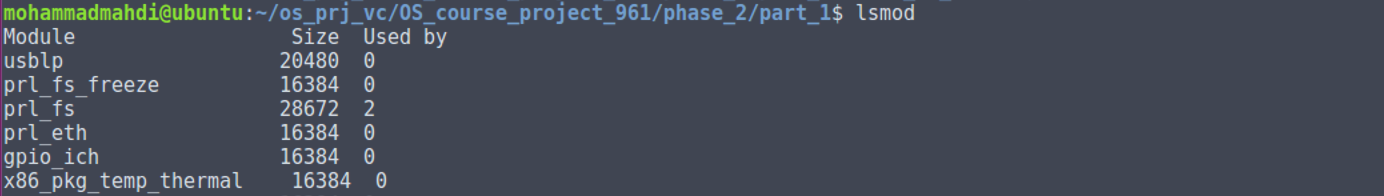
\includegraphics[width = 0.9\textwidth]{images/part_1/1.png}
	\caption{لیست ماژول‌های سیستم قبل از اضافه کردن ماژول ساخته شده}
\end{figure}


\begin{figure}[ht]
	\centering	
	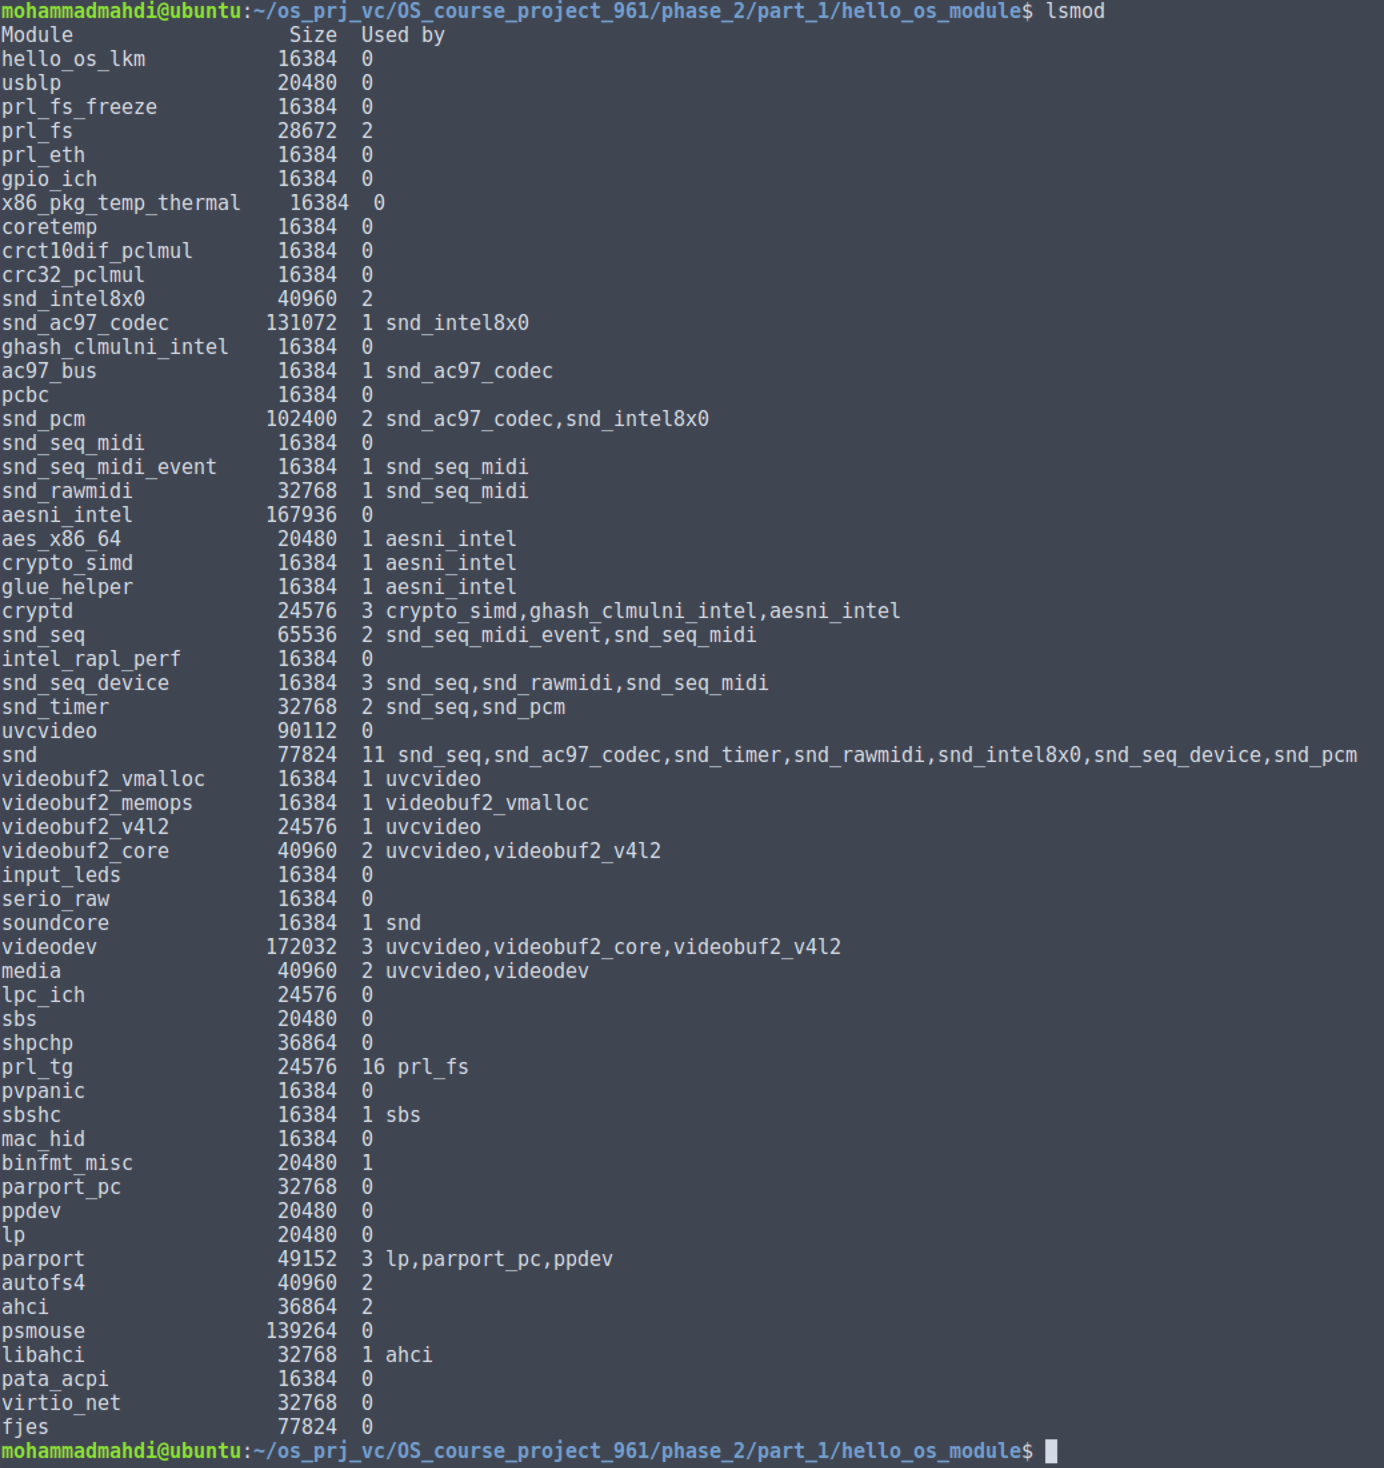
\includegraphics[width = 0.9\textwidth]{images/part_1/2.png}
	\caption{لیست ماژول‌های سیستم بعد از اضافه کردن ماژول ساخته شده}
\end{figure}


\begin{figure}[ht]
	\centering	
	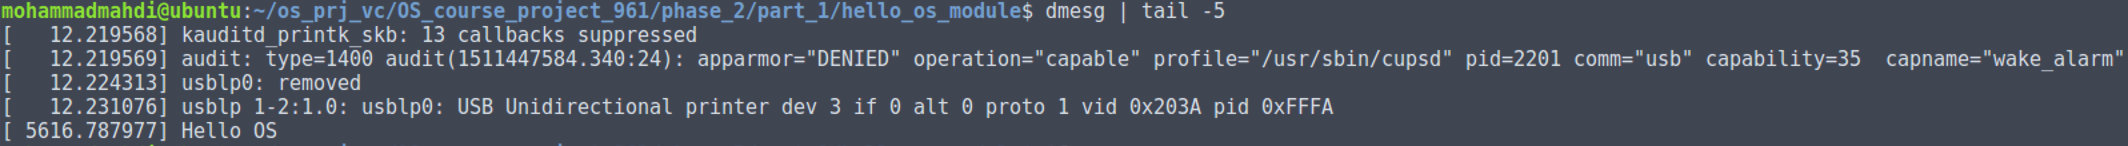
\includegraphics[width = 0.9\textwidth]{images/part_1/3.png}
	\caption{۵ خط پایانی خروجی دستور dmesg بعد از اضافه کردن ماژول ساخته شده}
\end{figure}


\begin{figure}[ht]
	\centering	
	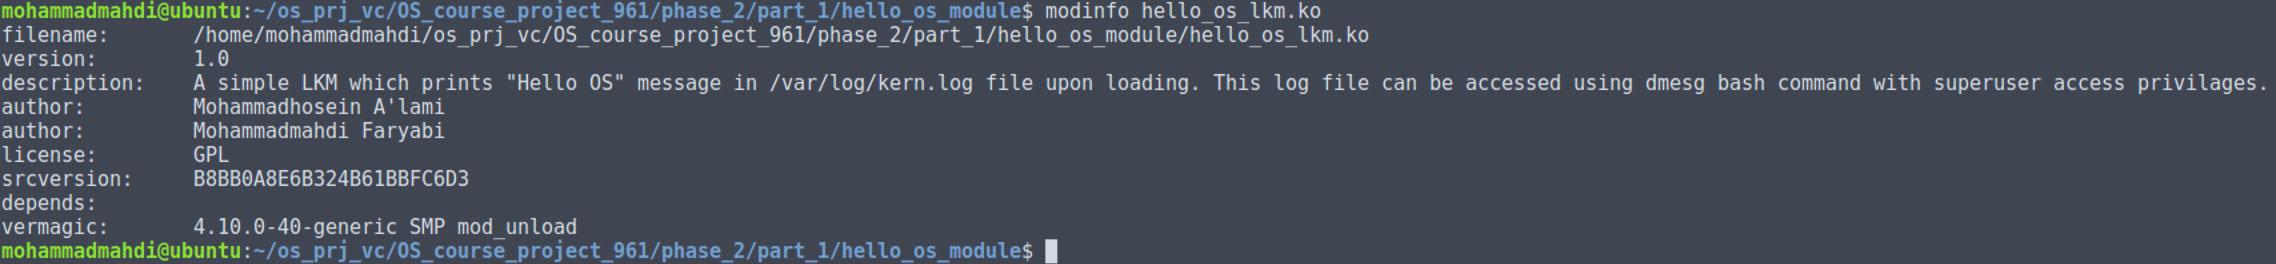
\includegraphics[width = 0.9\textwidth]{images/part_1/4.png}
	\caption{توضیحات ماژول ساخته‌شده}
\end{figure}



\section*{گام دوم: پیکره‌بندی و وصله کردن ماژول‌ها}

در این گام ابتدا فایل‌های زیر در کنار هم در یک دایرکتوری قرار می‌دهیم:

\begin{latin}
\begin{verbatim}
config-4.9.24-generic
grsecurity-3.1-4.9.24-201704252333.patch
grsecurity-3.1-4.9.24-201704252333.patch.sig
linux-4.9.24.tar.xz
\end{verbatim}
\end{latin}
توضیح در مورد این فایل‌‌ها که فایل \lr{linux-4.9.24.tar.xz} کد فشرده شده کرنل لینوکس است، فایل \lr{config-4.9.24-generic} مربوط به پیکربندی کرنل لینوکس است که می‌توان از آدرس /boot به آن دسترسی داشت. البته در این دایرکتوری فایل‌های پیکربندی کرنل‌های لینوکس فعال روی سیستم فعلی موجود است، که البته استفاده از پیکربندی‌های مختلف زیرمجموعه ورژن ۴ مشکلی ایجاد نخواهد کرد. فایل‌های مربوط به gresecurity به منظور اضافه کردن این پچ به کرنل استفاده می‌شوند که فایل .sig به نوعی امضای دیجیتالی فایل پچ است. 

حال به ترتیب زیر عمل می‌کنیم:

\begin{enumerate}

\item ابتدا فایل کرنل لینوکس را به کمک ابزار tar استخراج می‌کنیم

\begin{latin}
\begin{verbatim}
tar -xf linux-4.9.24.tar.xz
\end{verbatim}
\end{latin}

\item سپس به فولدر استخراج شده کرنل رفته و پچ grsecurity را به کرنل اضافه می‌کنیم.

\begin{latin}
\begin{verbatim}
cd linux-4.9.24/
patch -p1 < ../grsecurity-3.1-4.9.24-201704252333.patch
\end{verbatim}
\end{latin}

\item سپس فایل پیکربندی لینوکس را به فولدر استخراج شده می‌بریم و تغییرات پیکربندی را آغاز می‌کنیم.

\begin{latin}
\begin{verbatim}
cd ..
mv config-4.10.0-40-generic linux-4.9.24/.config
cd linux-4.9.24/
make menuconfig
\end{verbatim}
\end{latin}

\item با زدن دستور \lr{make menuconfig} منوی زیر برای پیکربندی کرنل بالا می‌آيد که به ترتیب زیر عمل می‌کنیم:

\newpage

\begin{figure}[ht]
	\centering	
	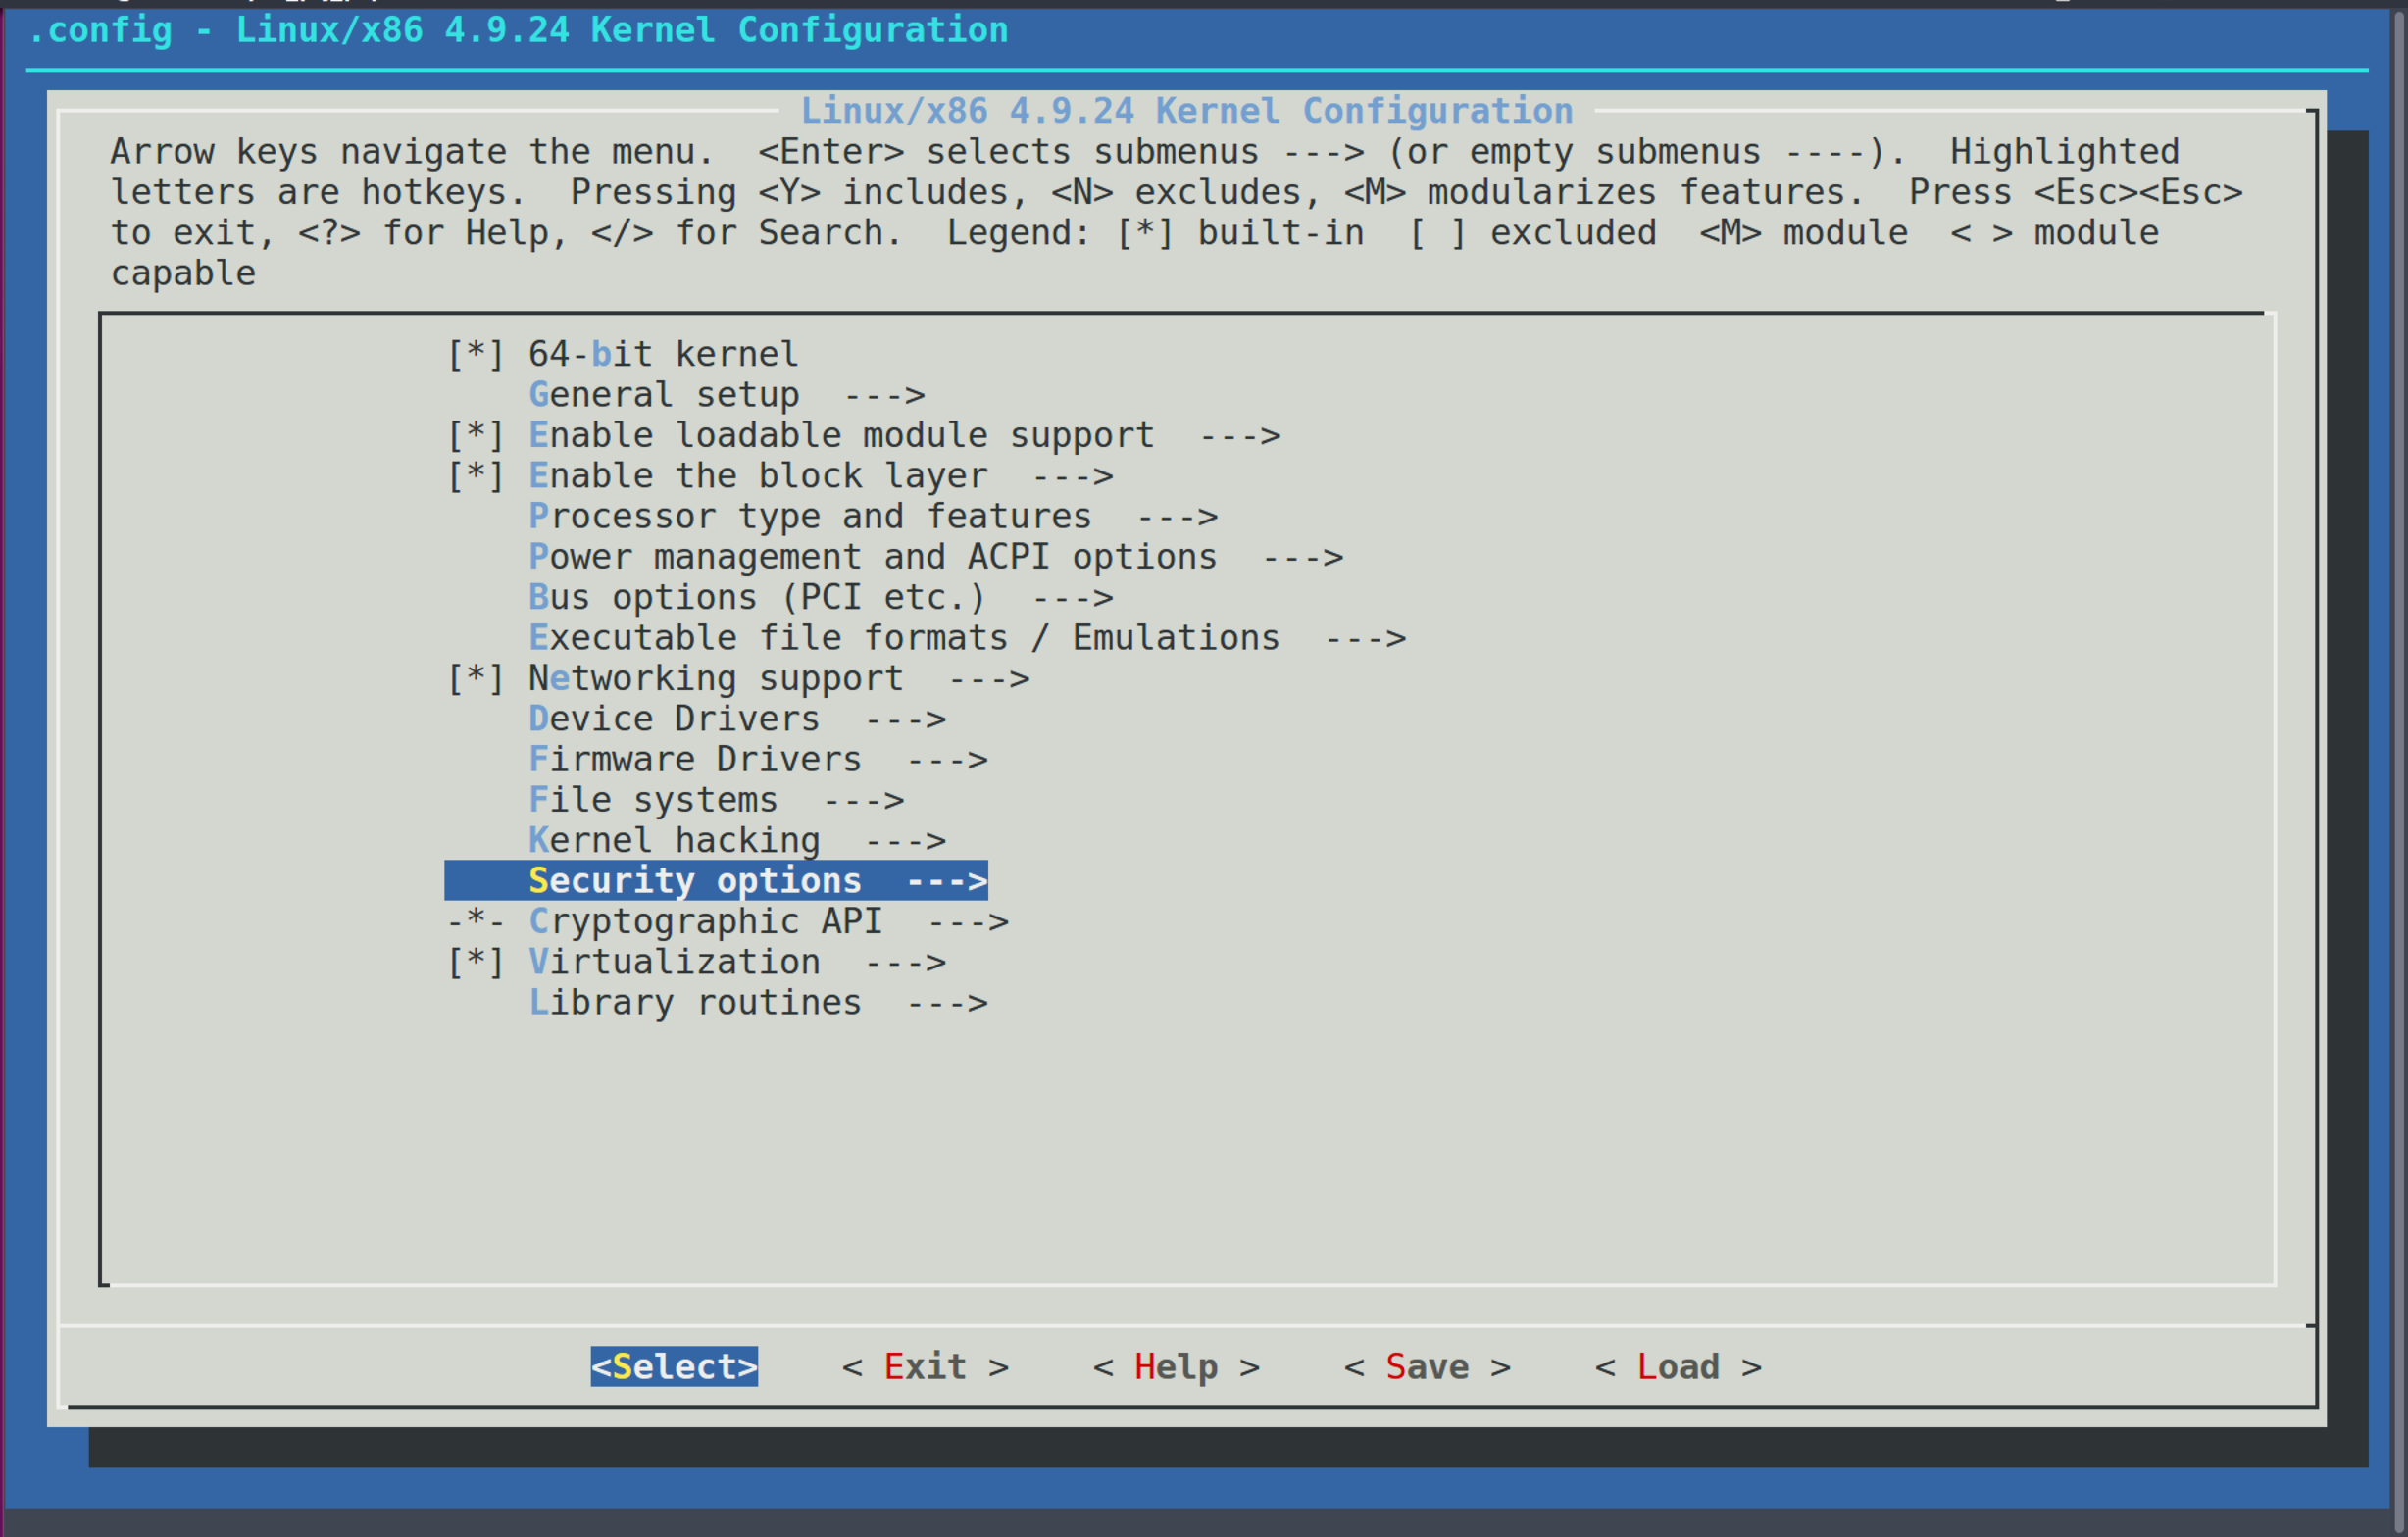
\includegraphics[width = 0.9\textwidth]{images/1.png}
\end{figure}
به قسمت \lr{Security options} می‌رویم.
\begin{figure}[ht]
	\centering	
	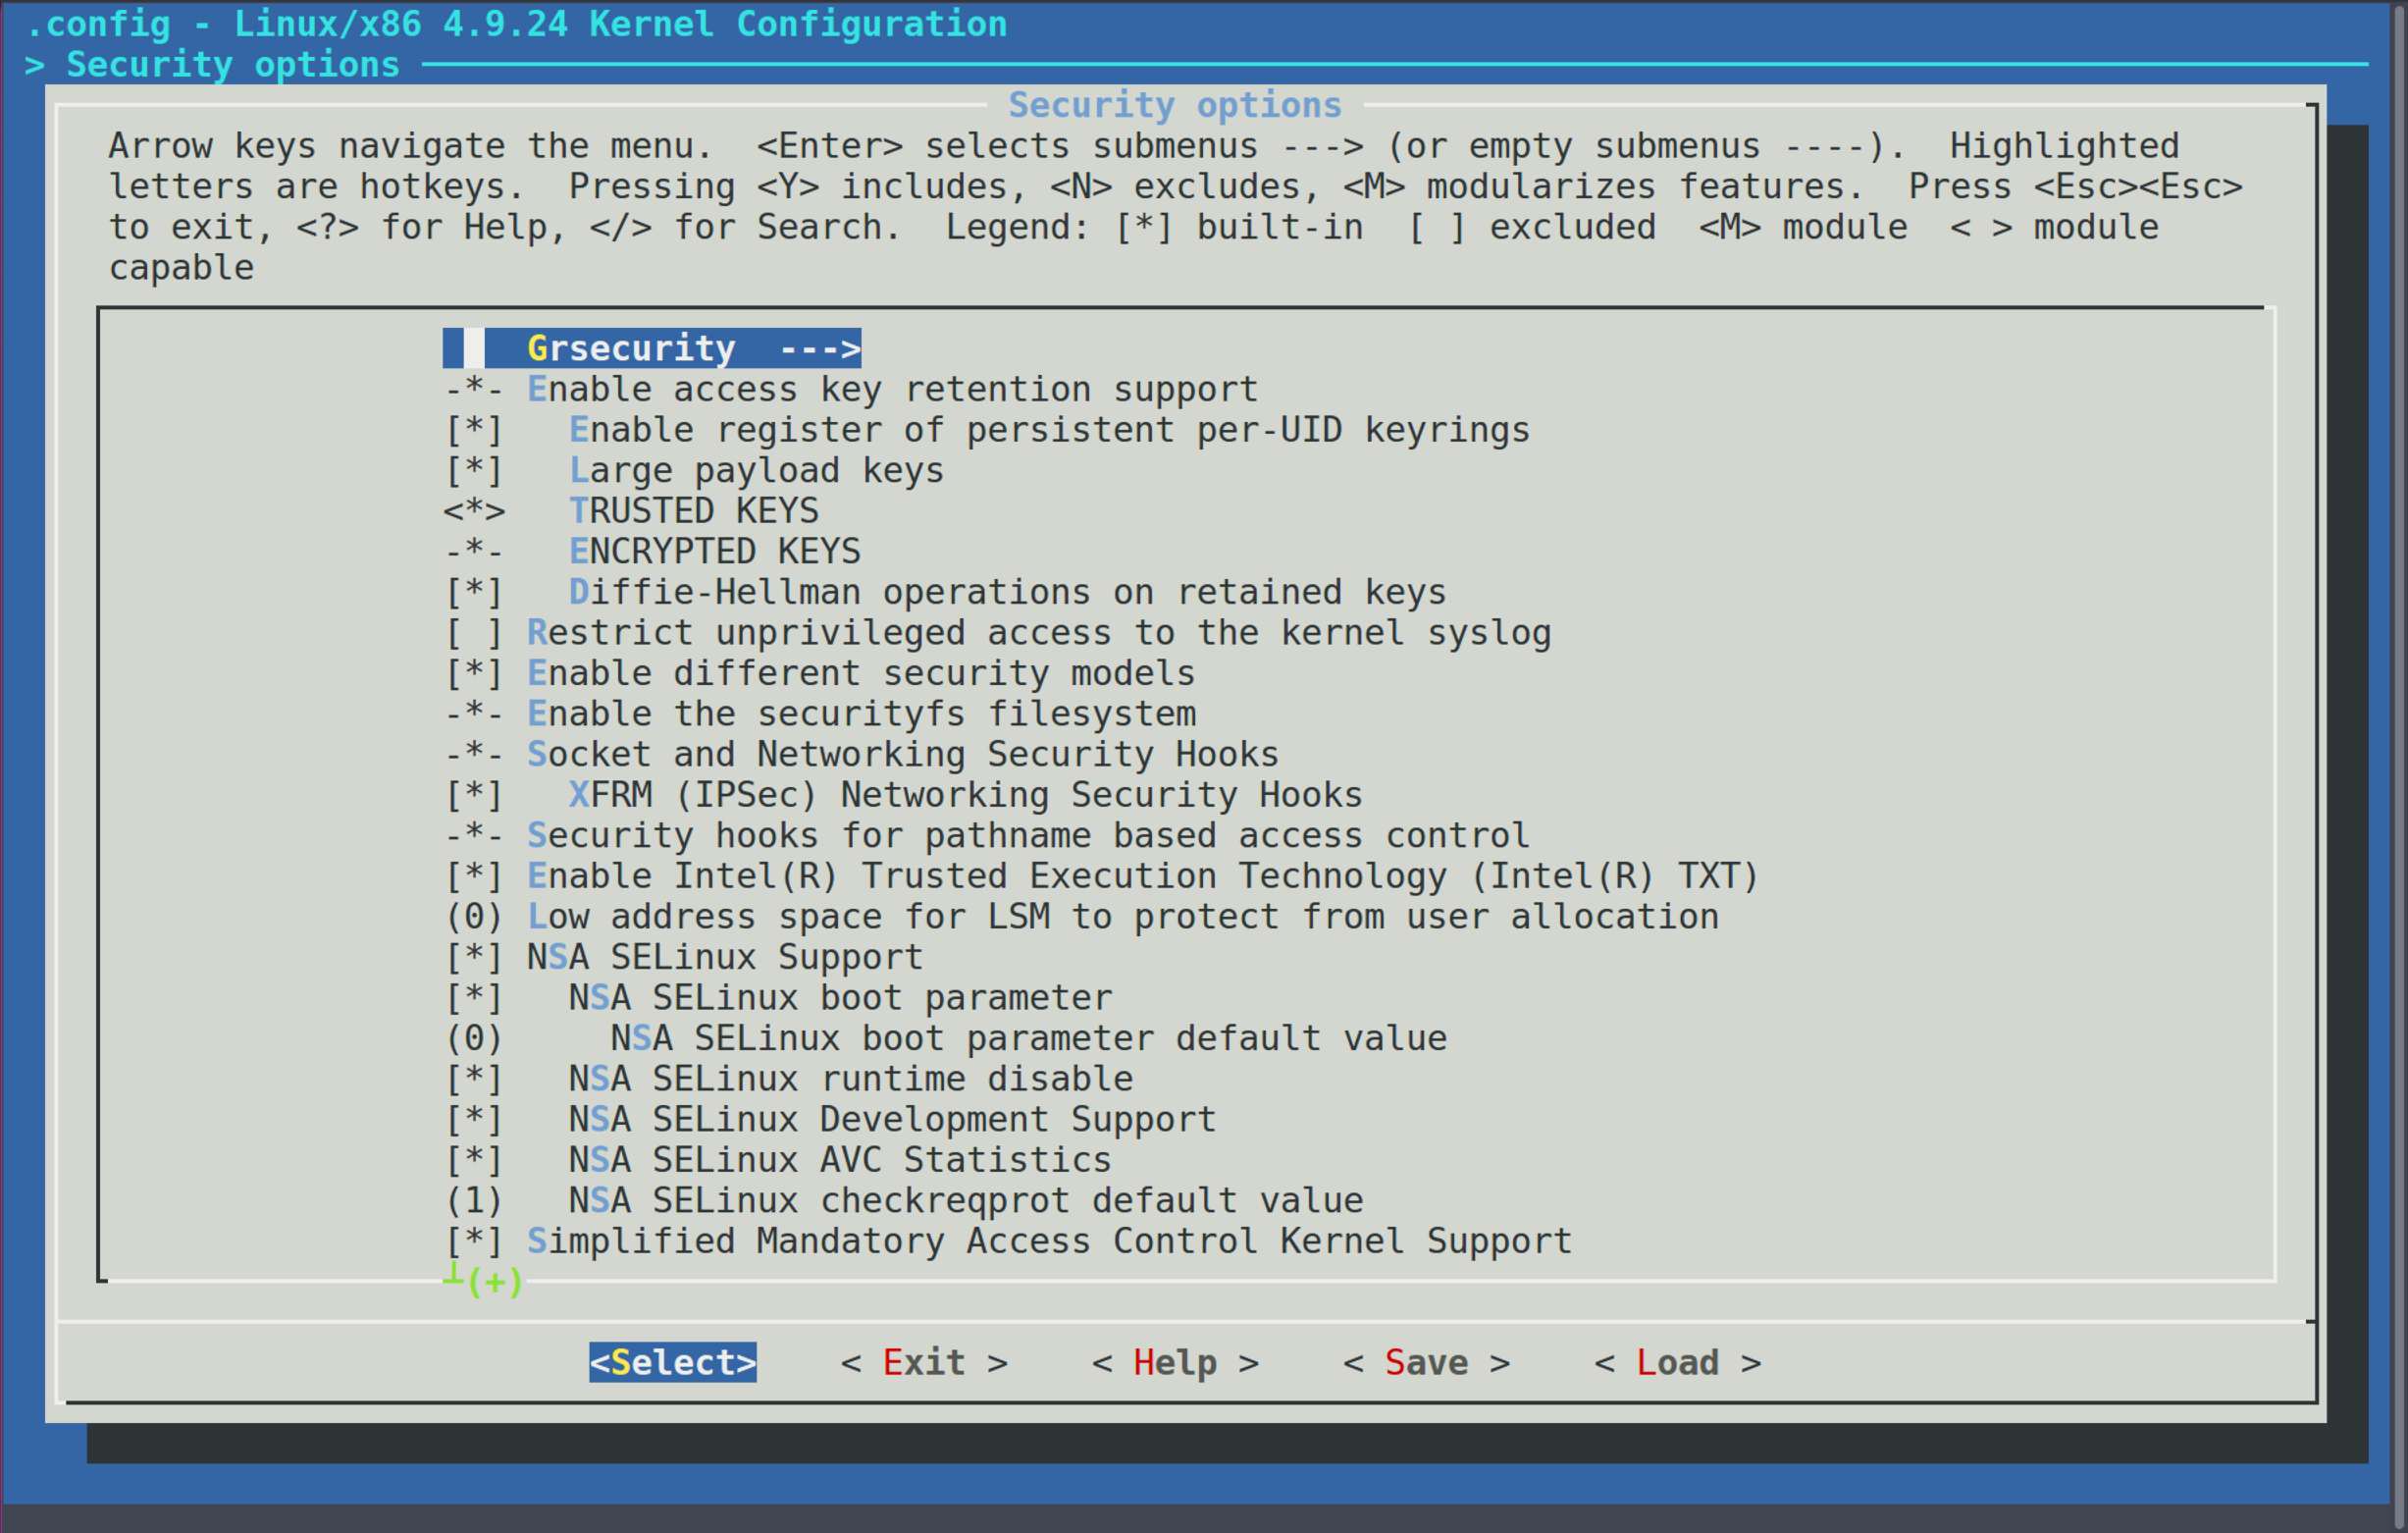
\includegraphics[width = 0.9\textwidth]{images/2.png}
\end{figure}

سپس به قسمت Grsecurity می‌رویم.
\newpage
\begin{figure}[ht]
	\centering	
	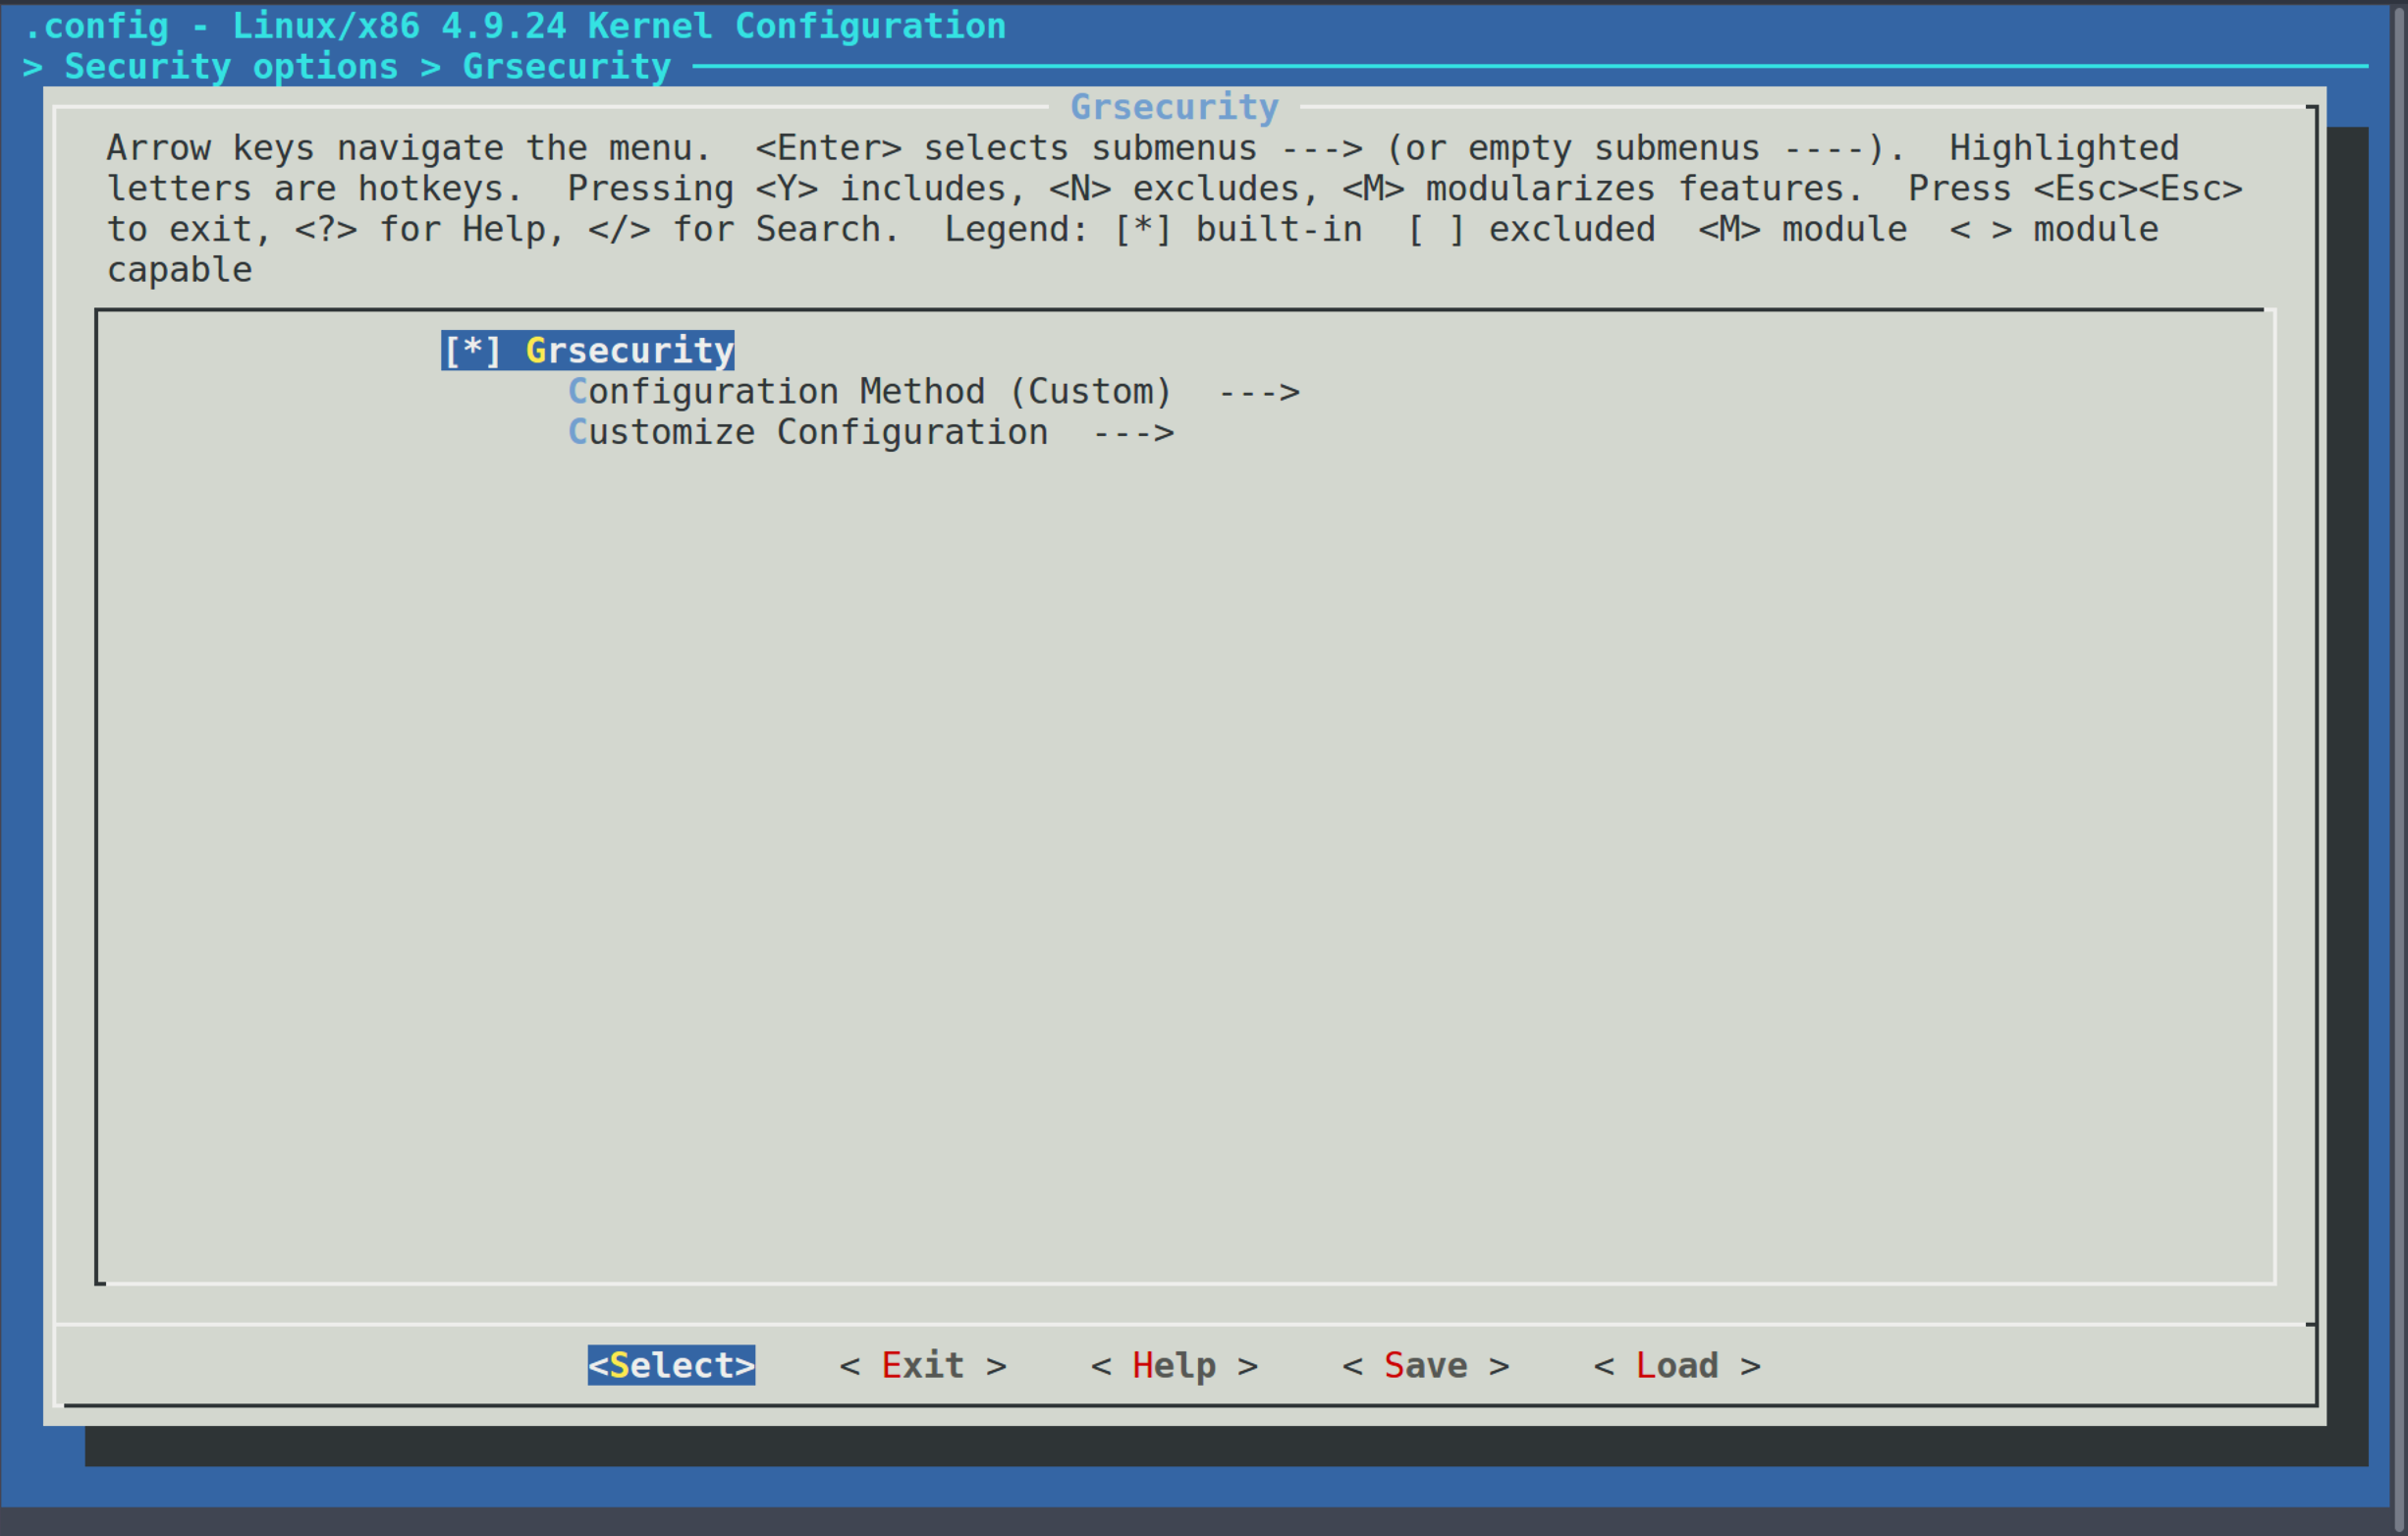
\includegraphics[width = 0.9\textwidth]{images/3.png}
\end{figure}

سپس به Configuration Method می‌رویم.
\begin{figure}[ht]
	\centering	
	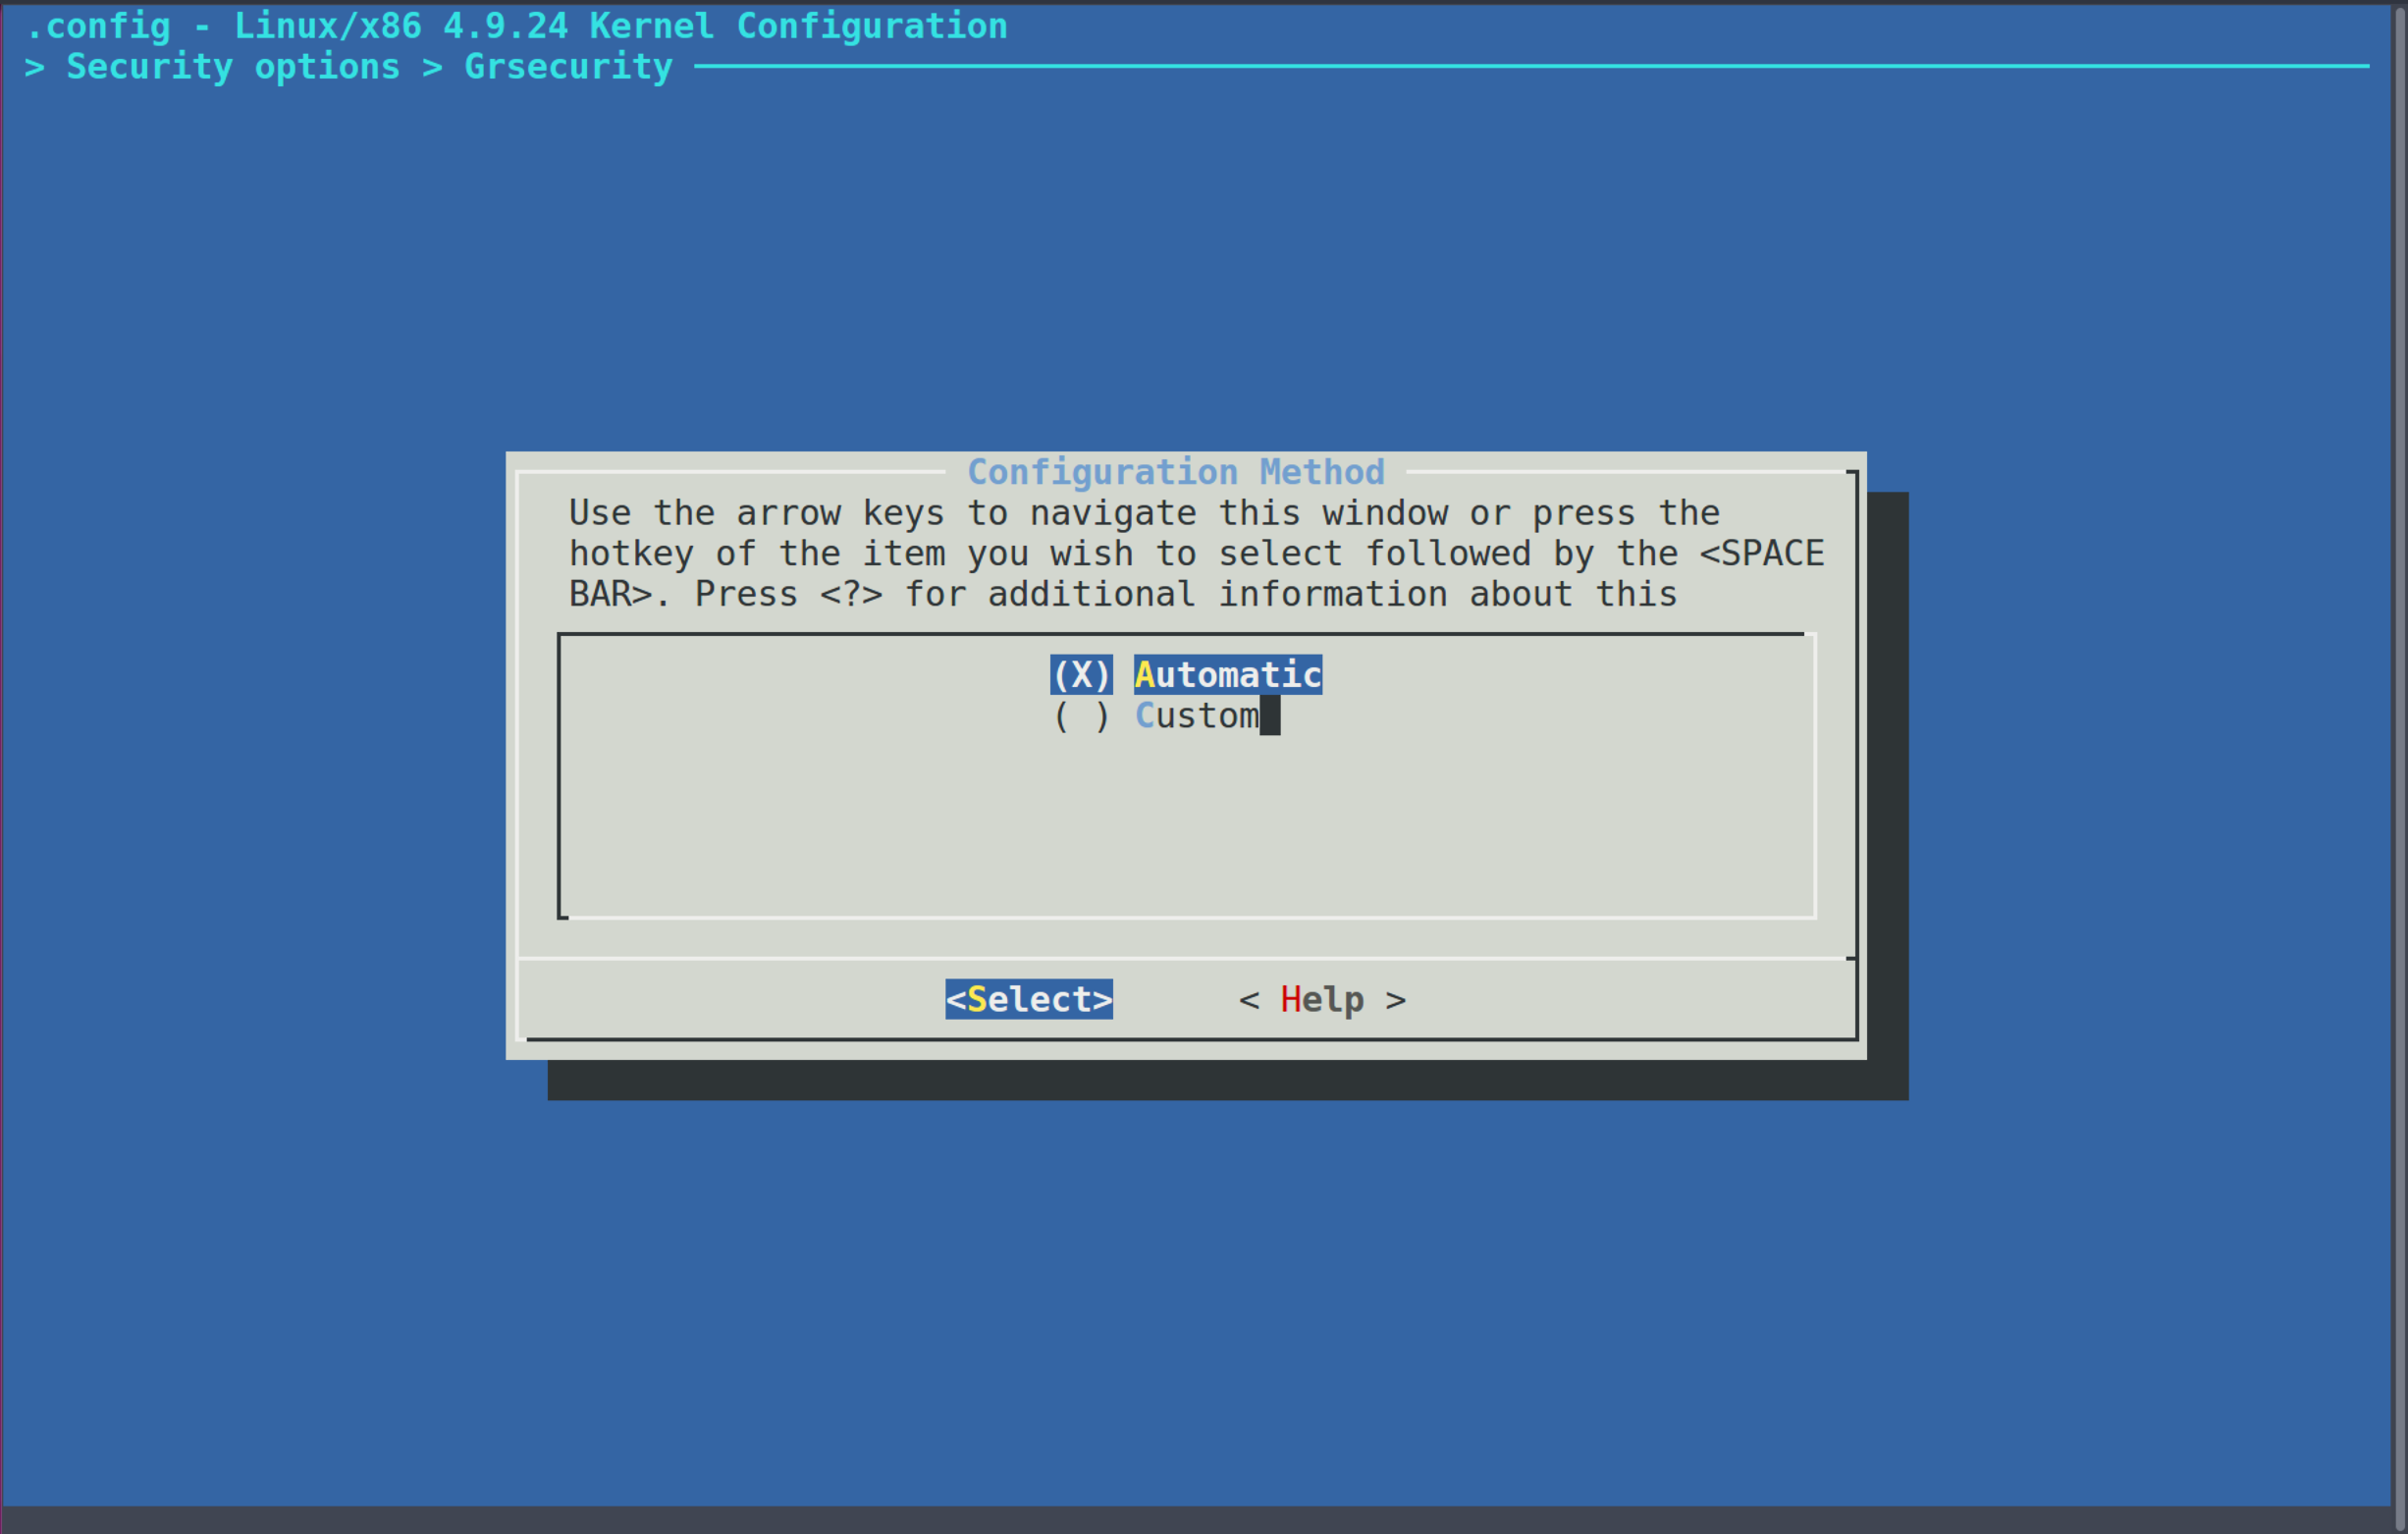
\includegraphics[width = 0.9\textwidth]{images/4.png}
\end{figure}

و گزینه Automatic را انتخاب می‌کنیم. زمانی که به منوی قبلی برمی‌گردیم این منو گسترش یافته است.

\newpage
\begin{figure}[ht]
	\centering	
	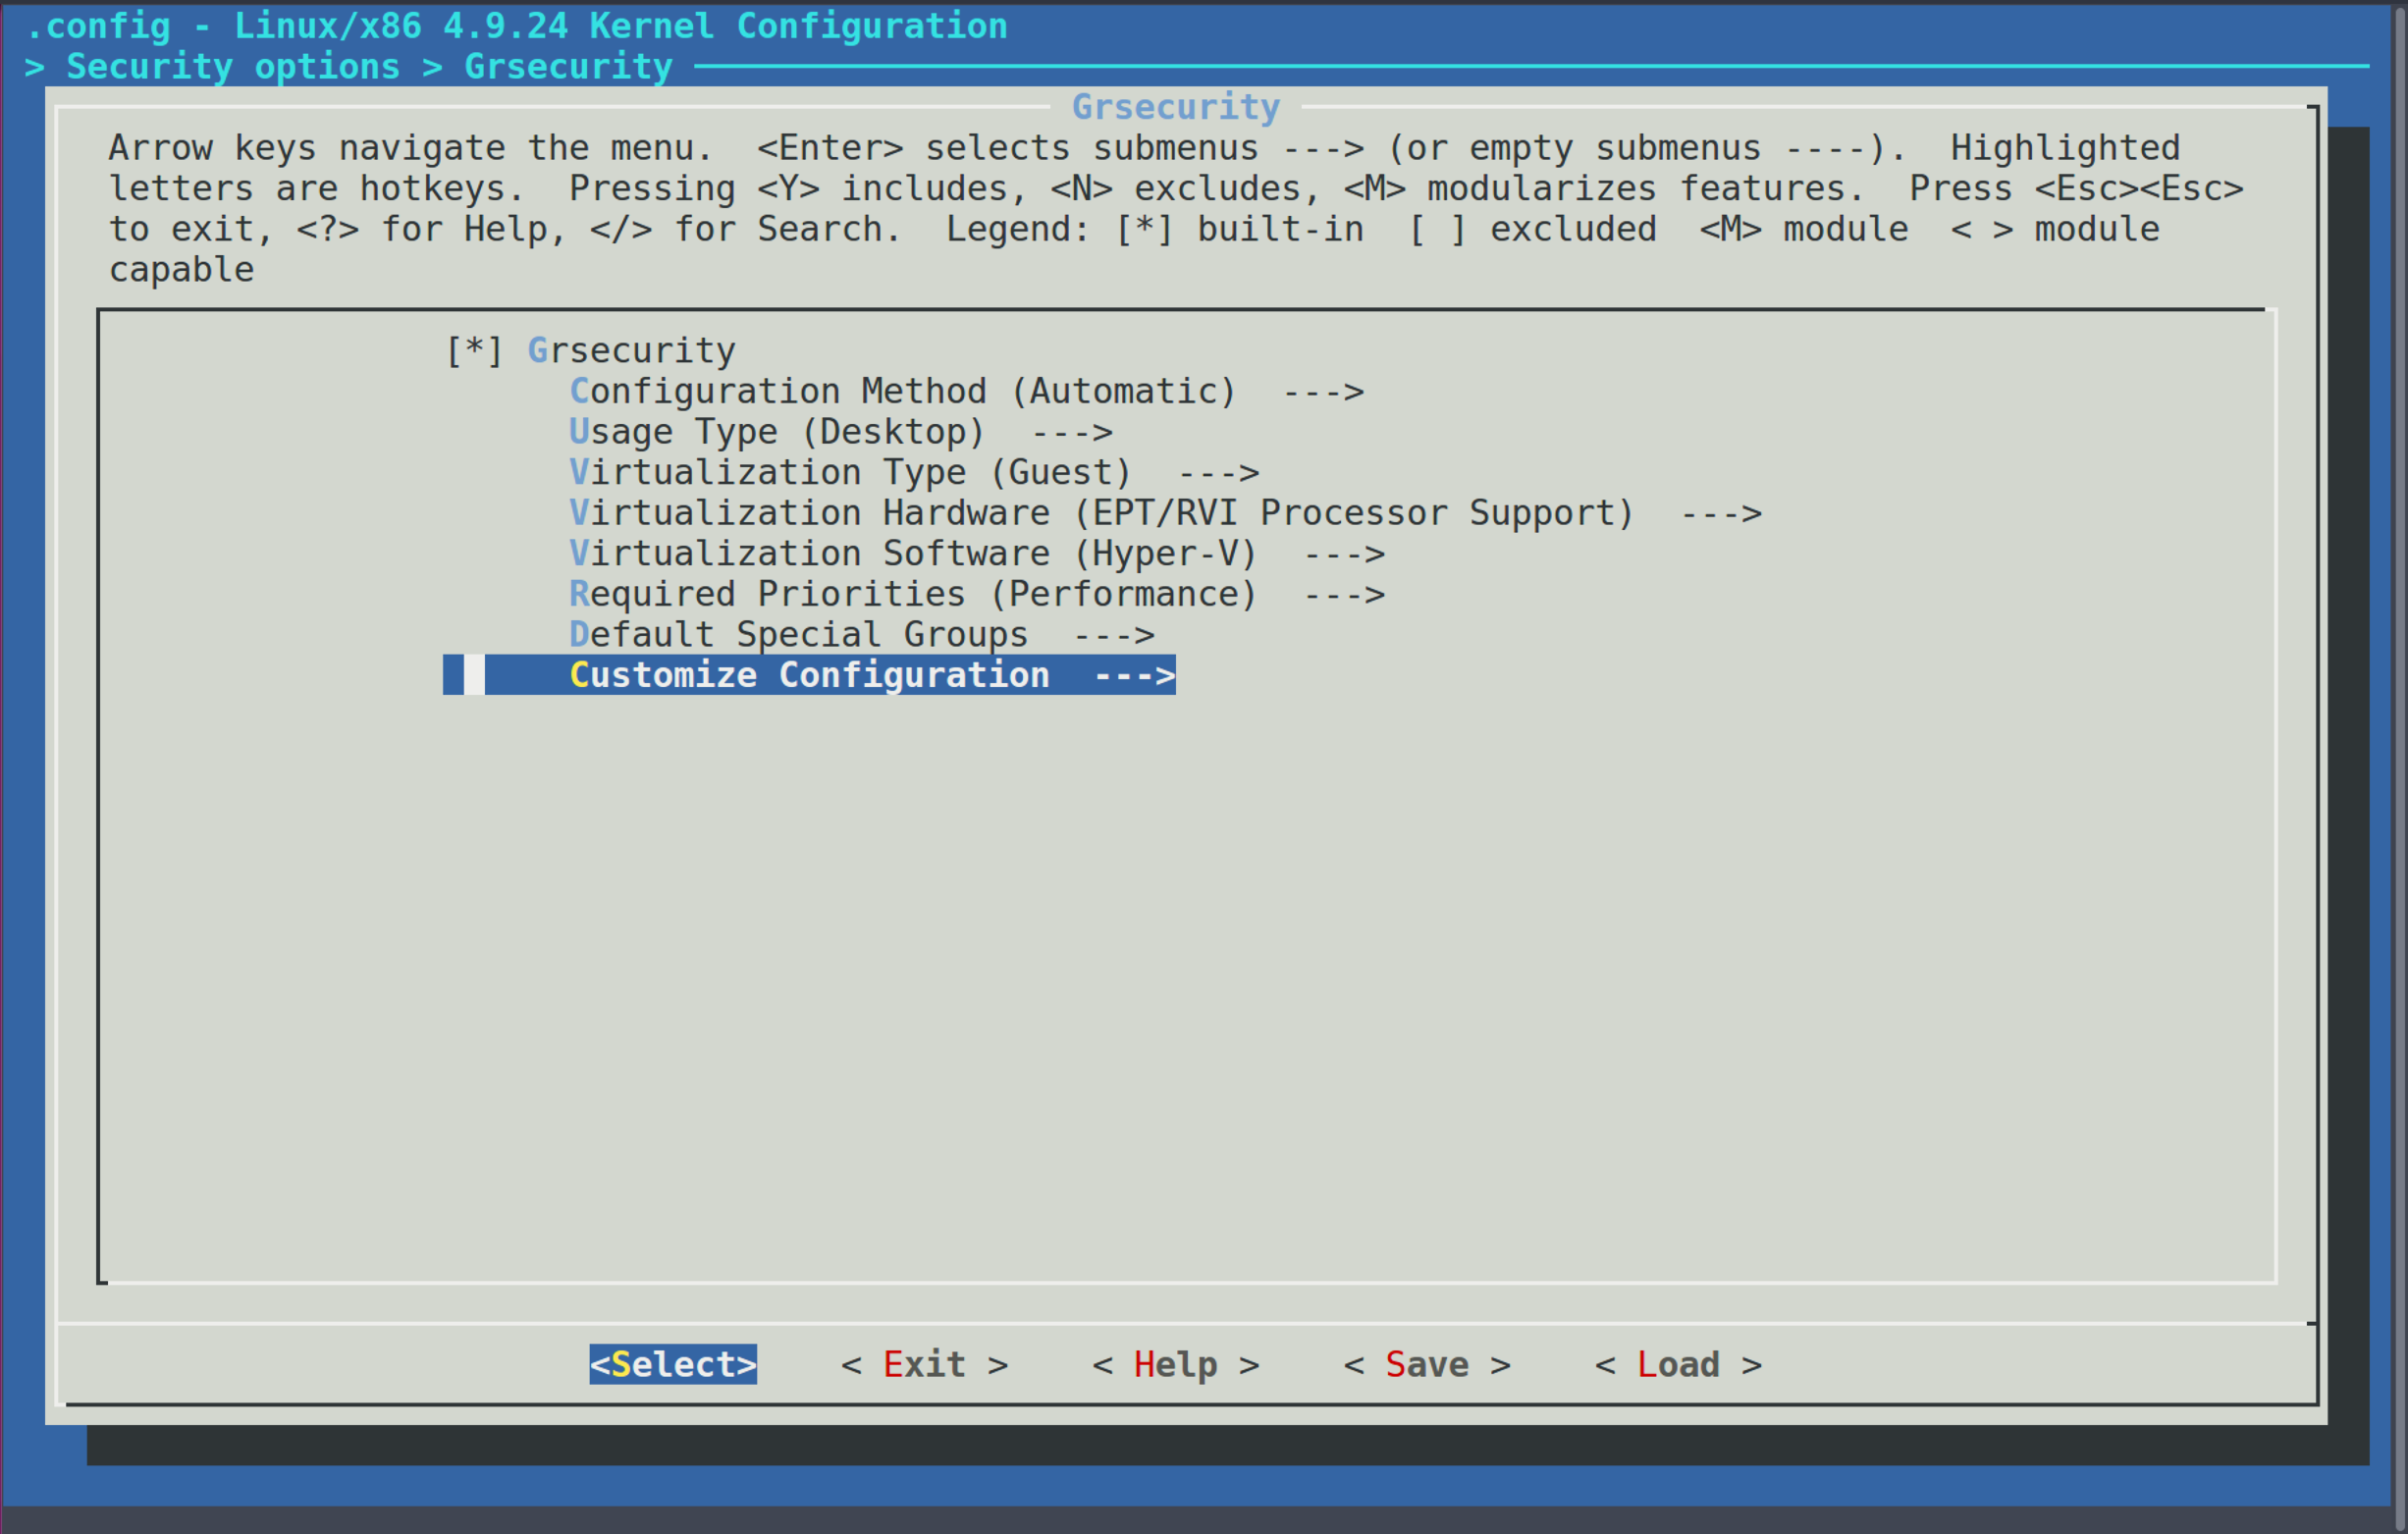
\includegraphics[width = 0.9\textwidth]{images/5.png}
\end{figure}
سپس به ترتیب هر کدام از پیکر‌بندی‌های موجود در لیست را به شکل زیر تغییر می‌دهیم:
\begin{figure}[ht]
	\centering	
	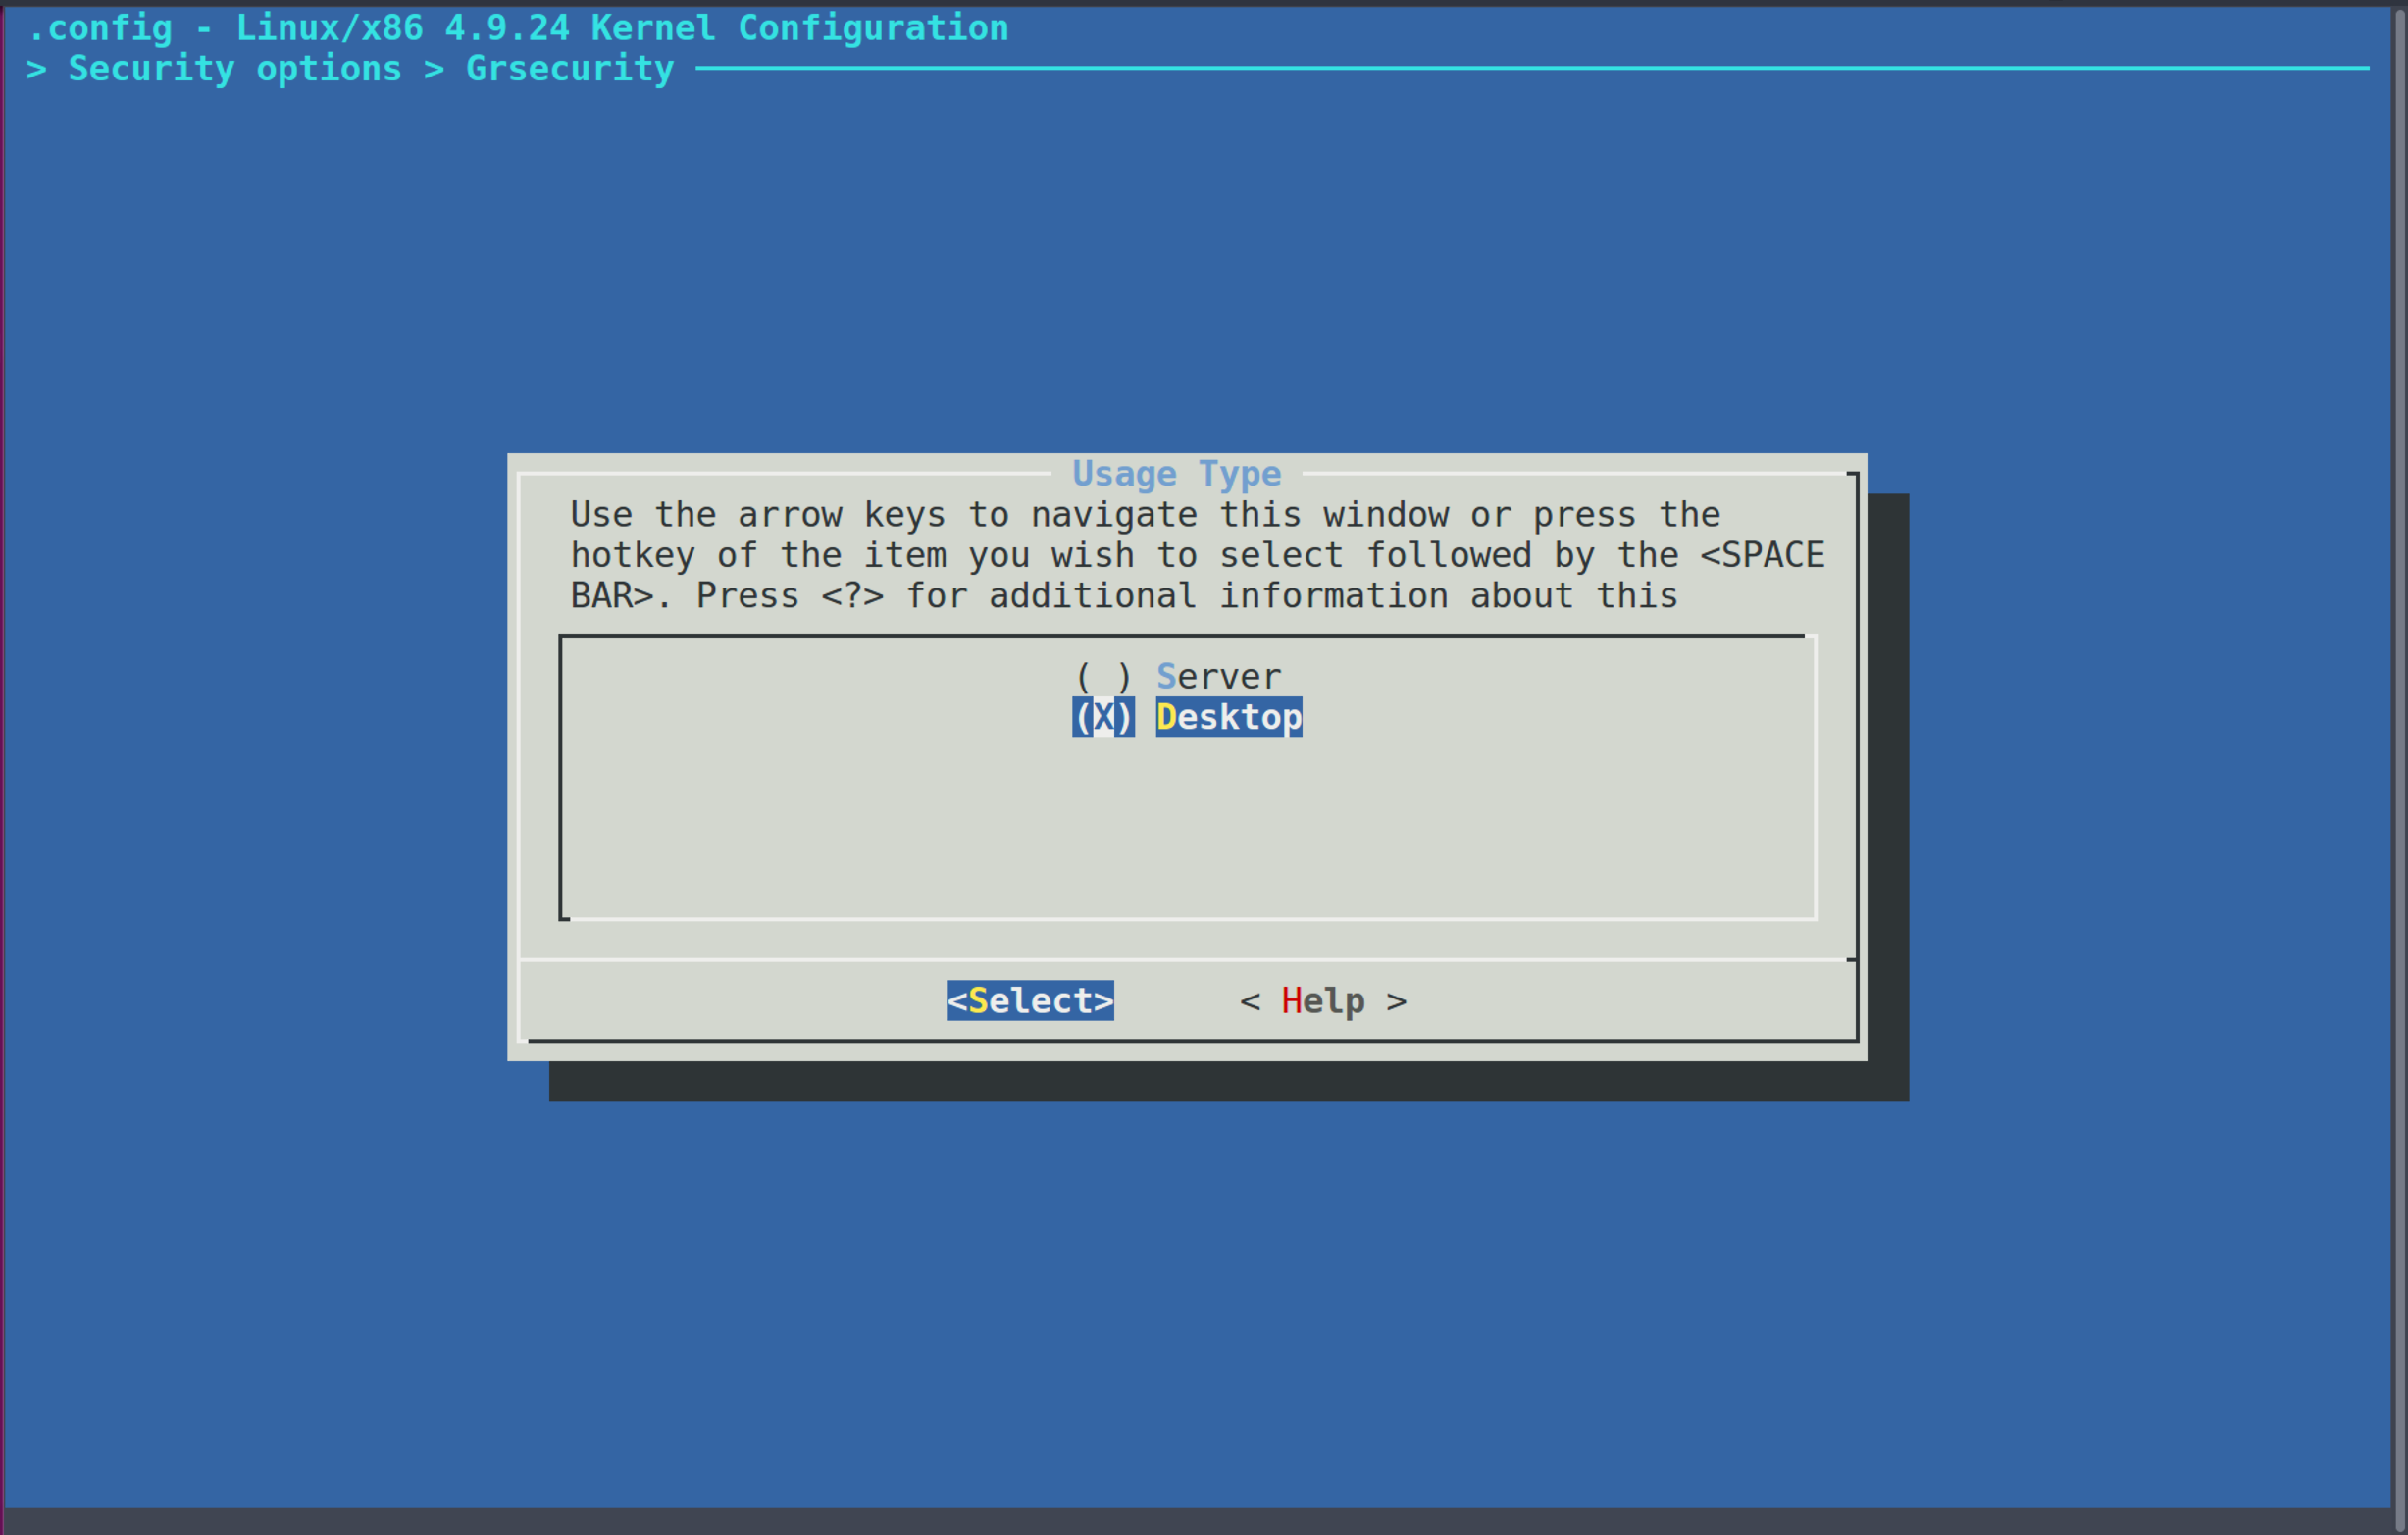
\includegraphics[width = 0.9\textwidth]{images/6.png}
\end{figure}
\newpage
\begin{figure}[ht]
	\centering	
	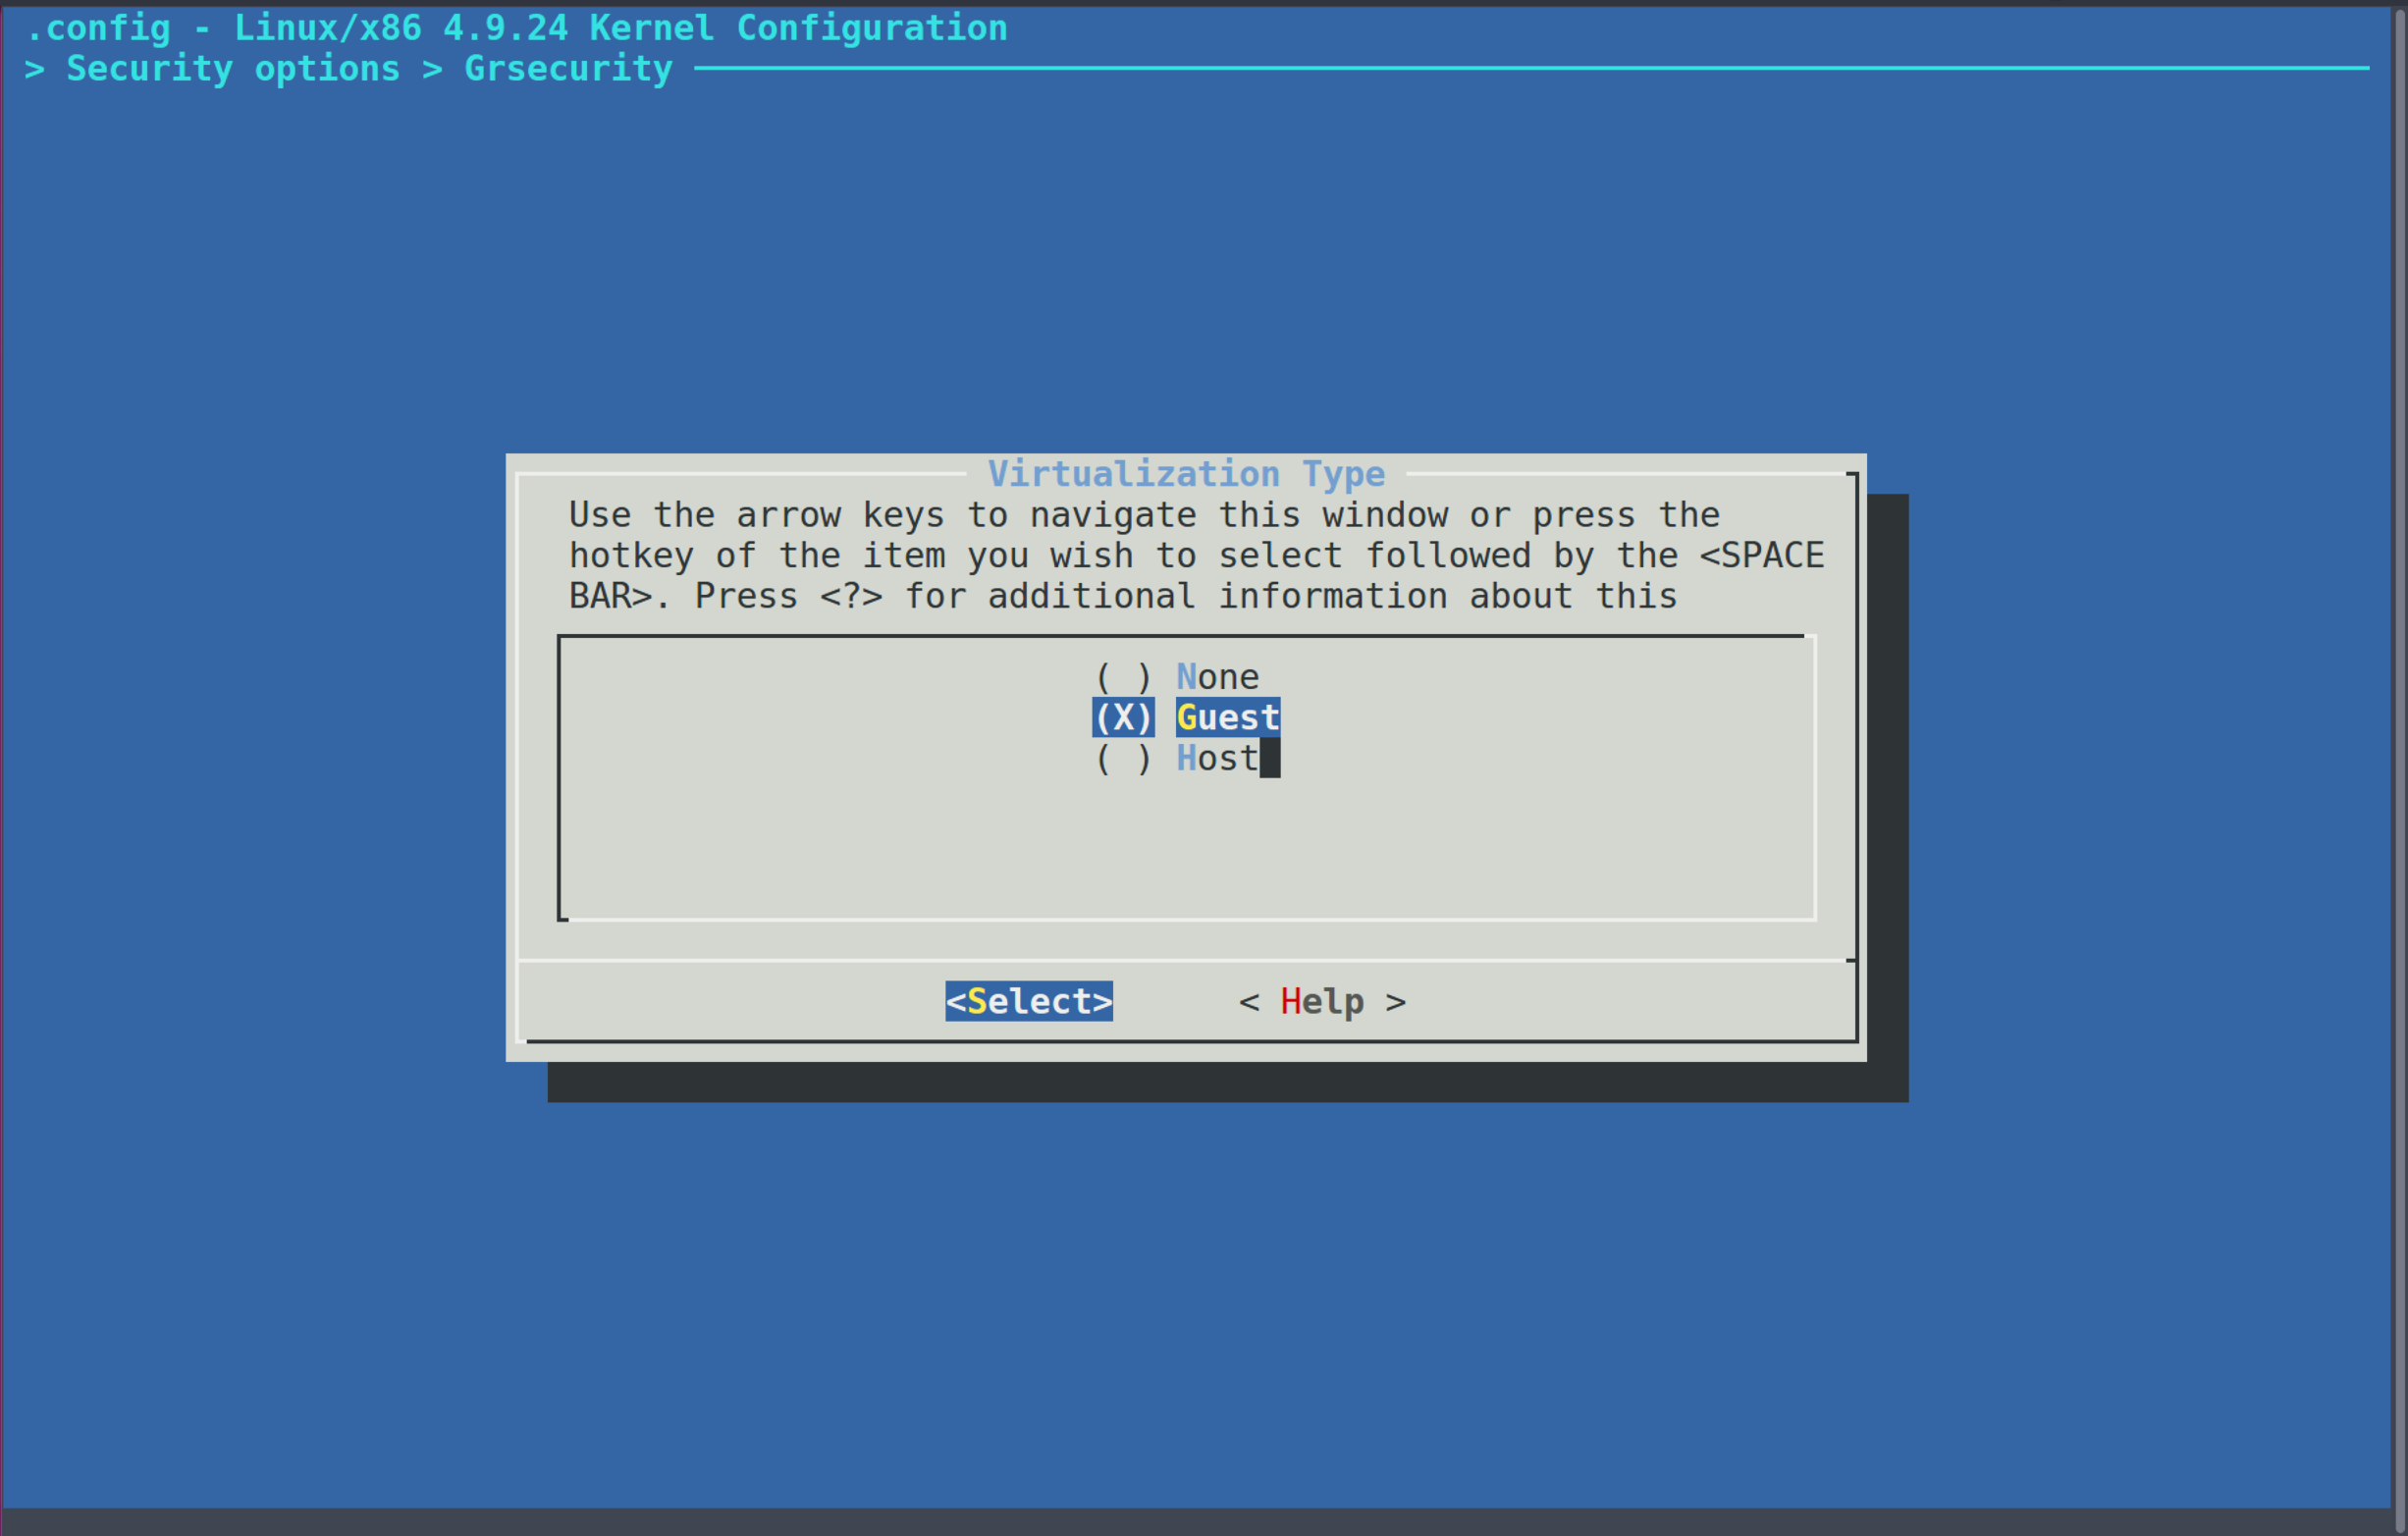
\includegraphics[width = 0.9\textwidth]{images/7.png}
\end{figure}
\begin{figure}[ht]
	\centering	
	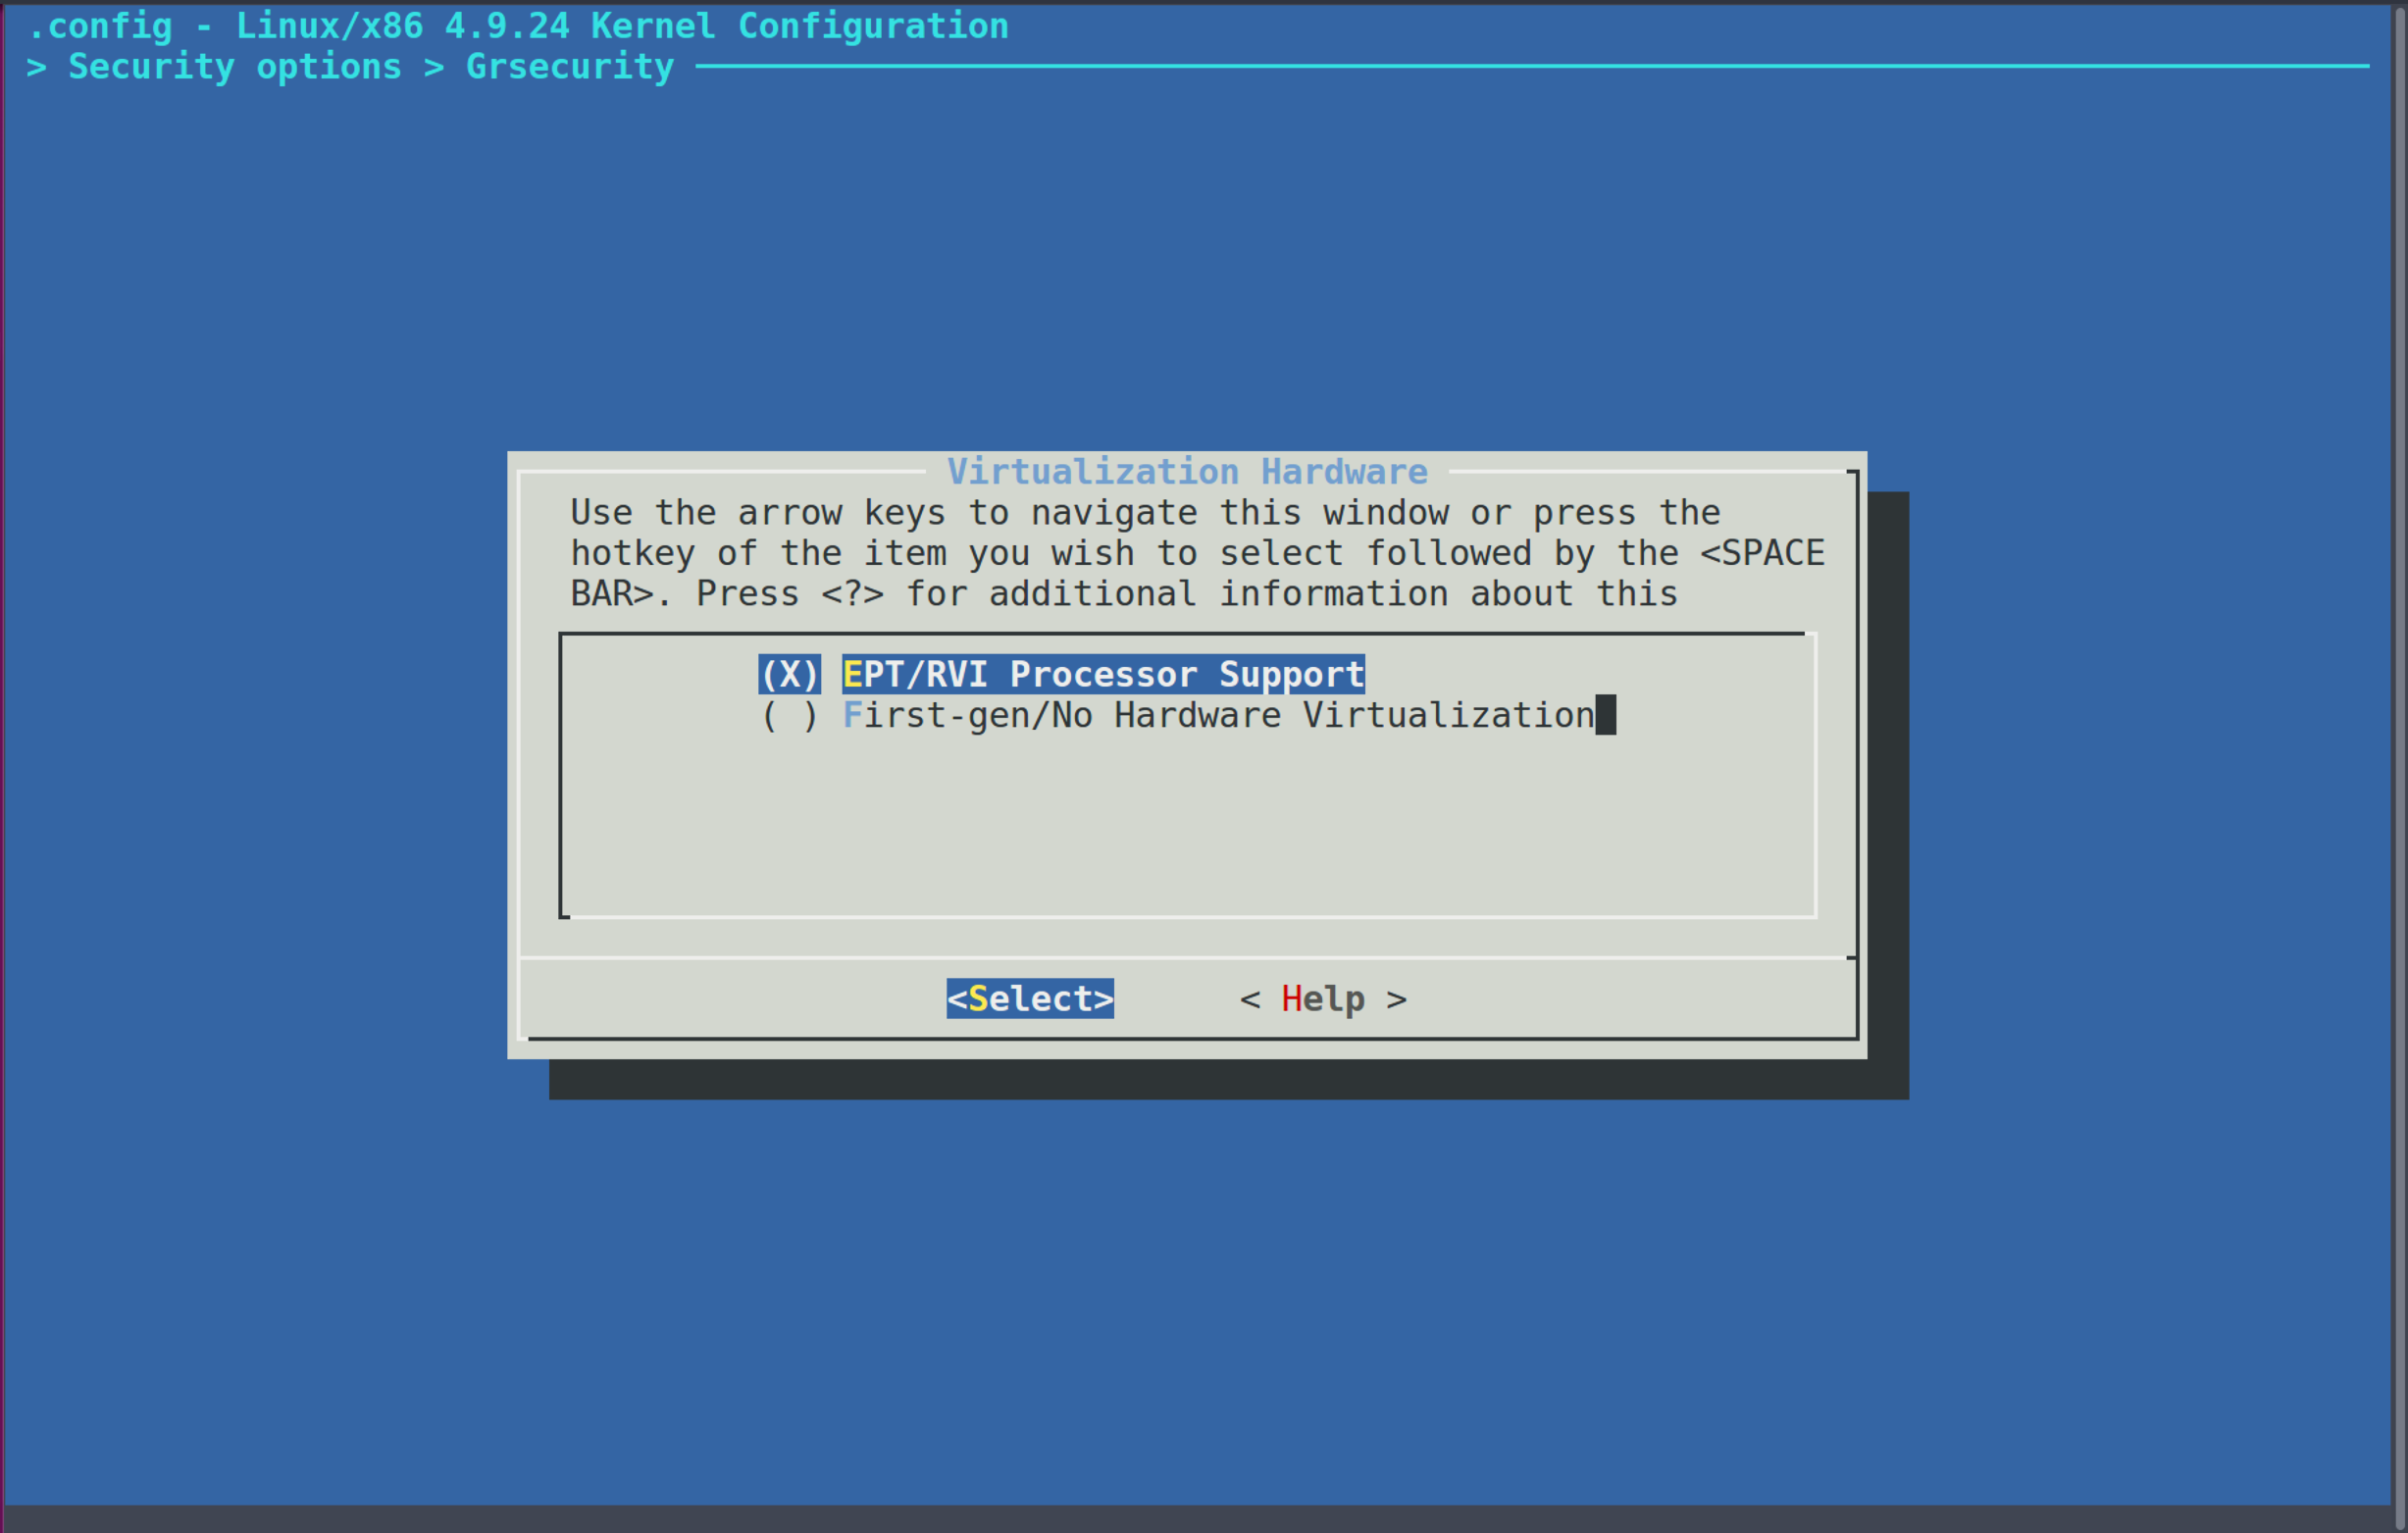
\includegraphics[width = 0.9\textwidth]{images/8.png}
\end{figure}
\newpage
\begin{figure}[ht]
	\centering	
	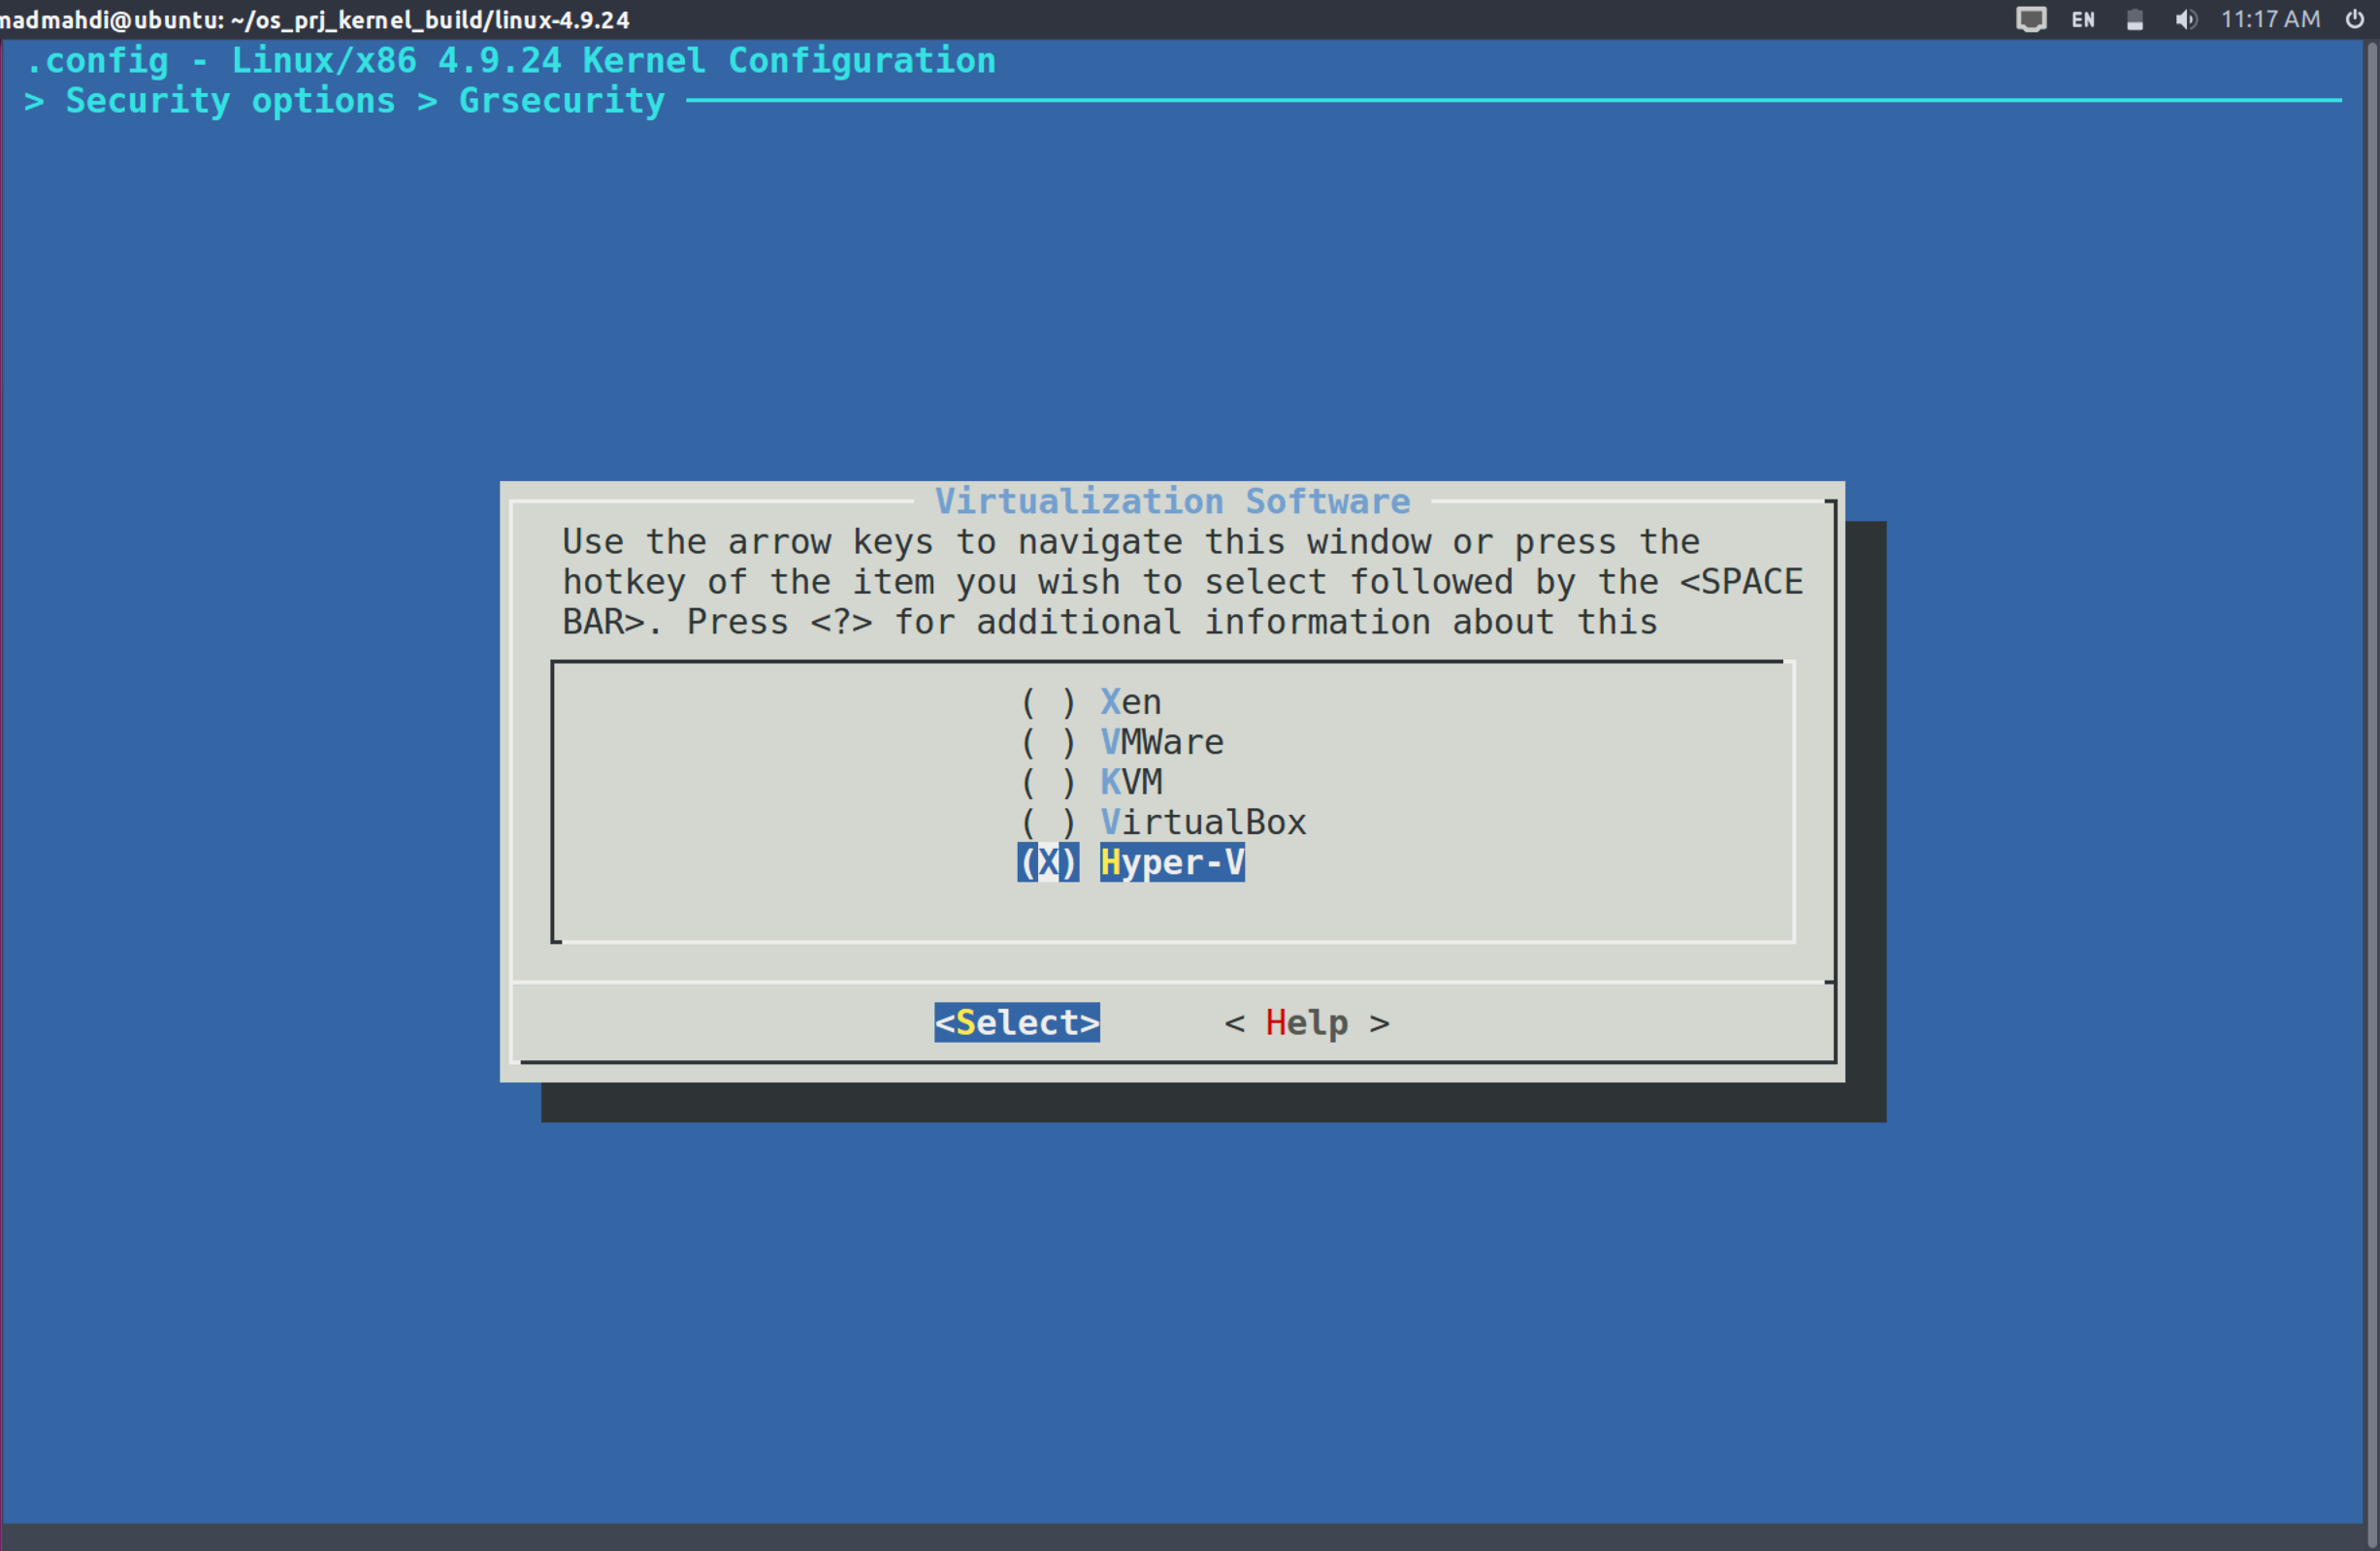
\includegraphics[width = 0.9\textwidth]{images/9.png}
\end{figure}
\begin{figure}[ht]
	\centering	
	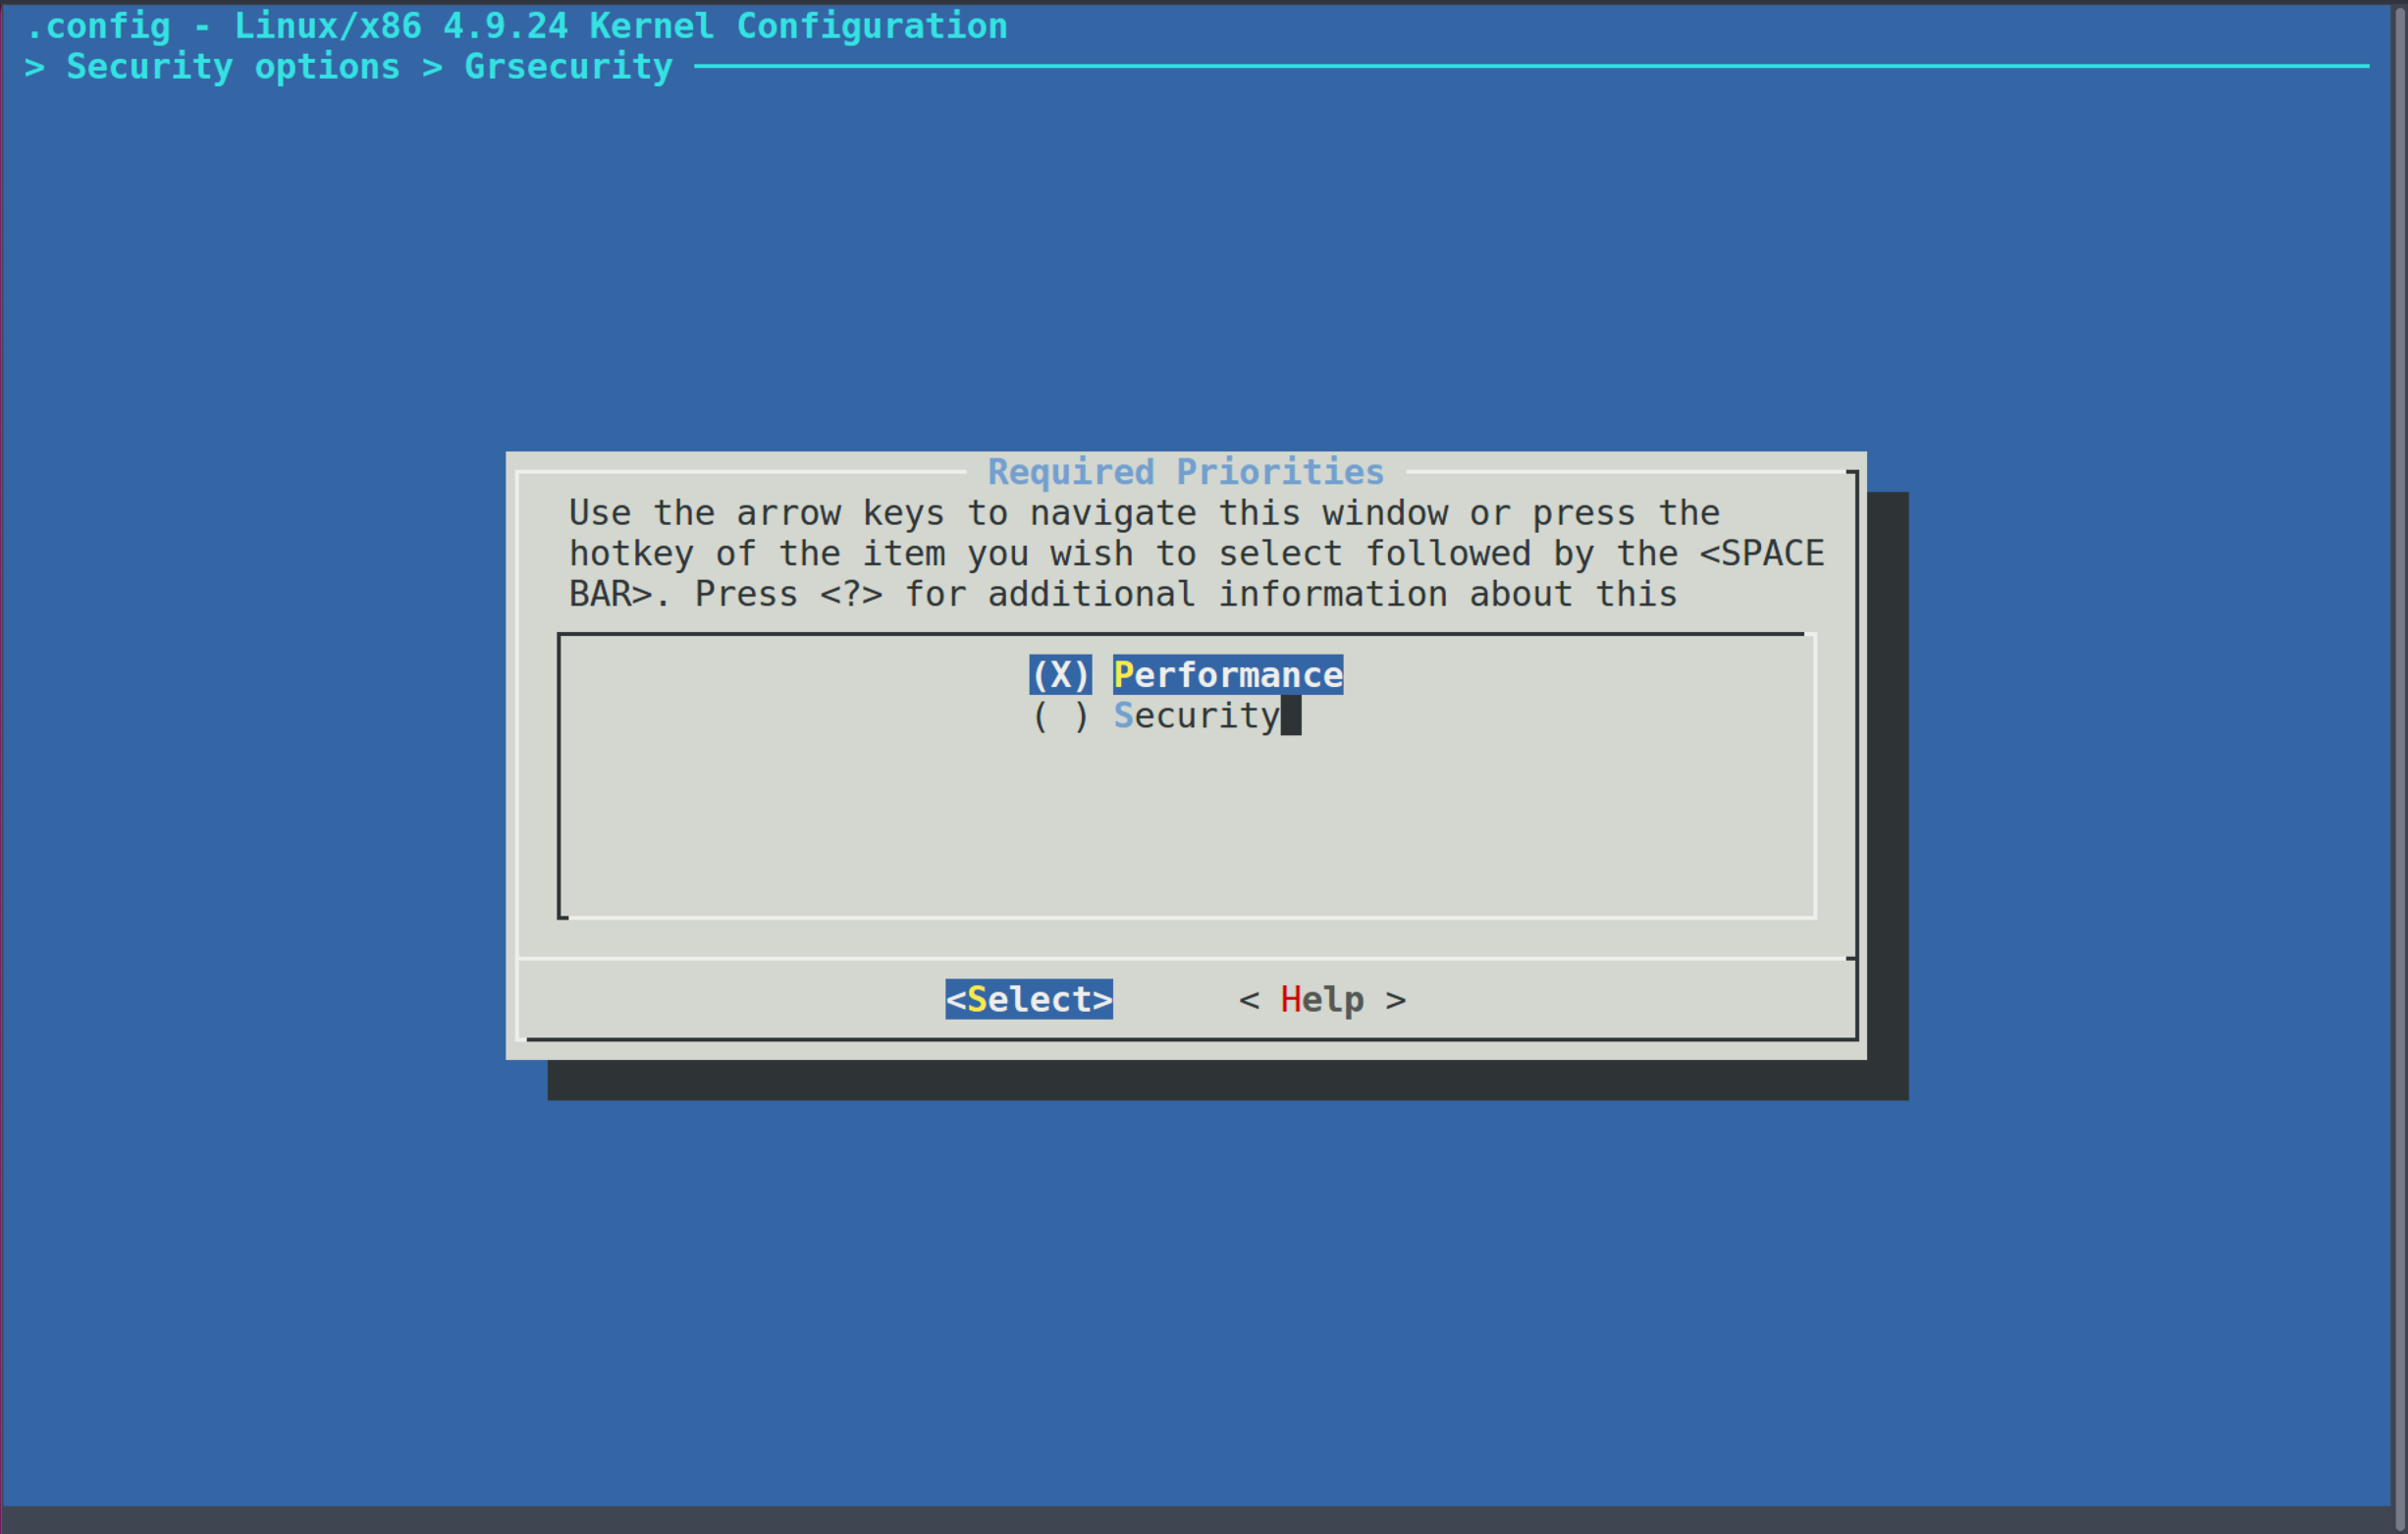
\includegraphics[width = 0.9\textwidth]{images/10.png}
\end{figure}
\newpage
\begin{figure}[ht]
	\centering	
	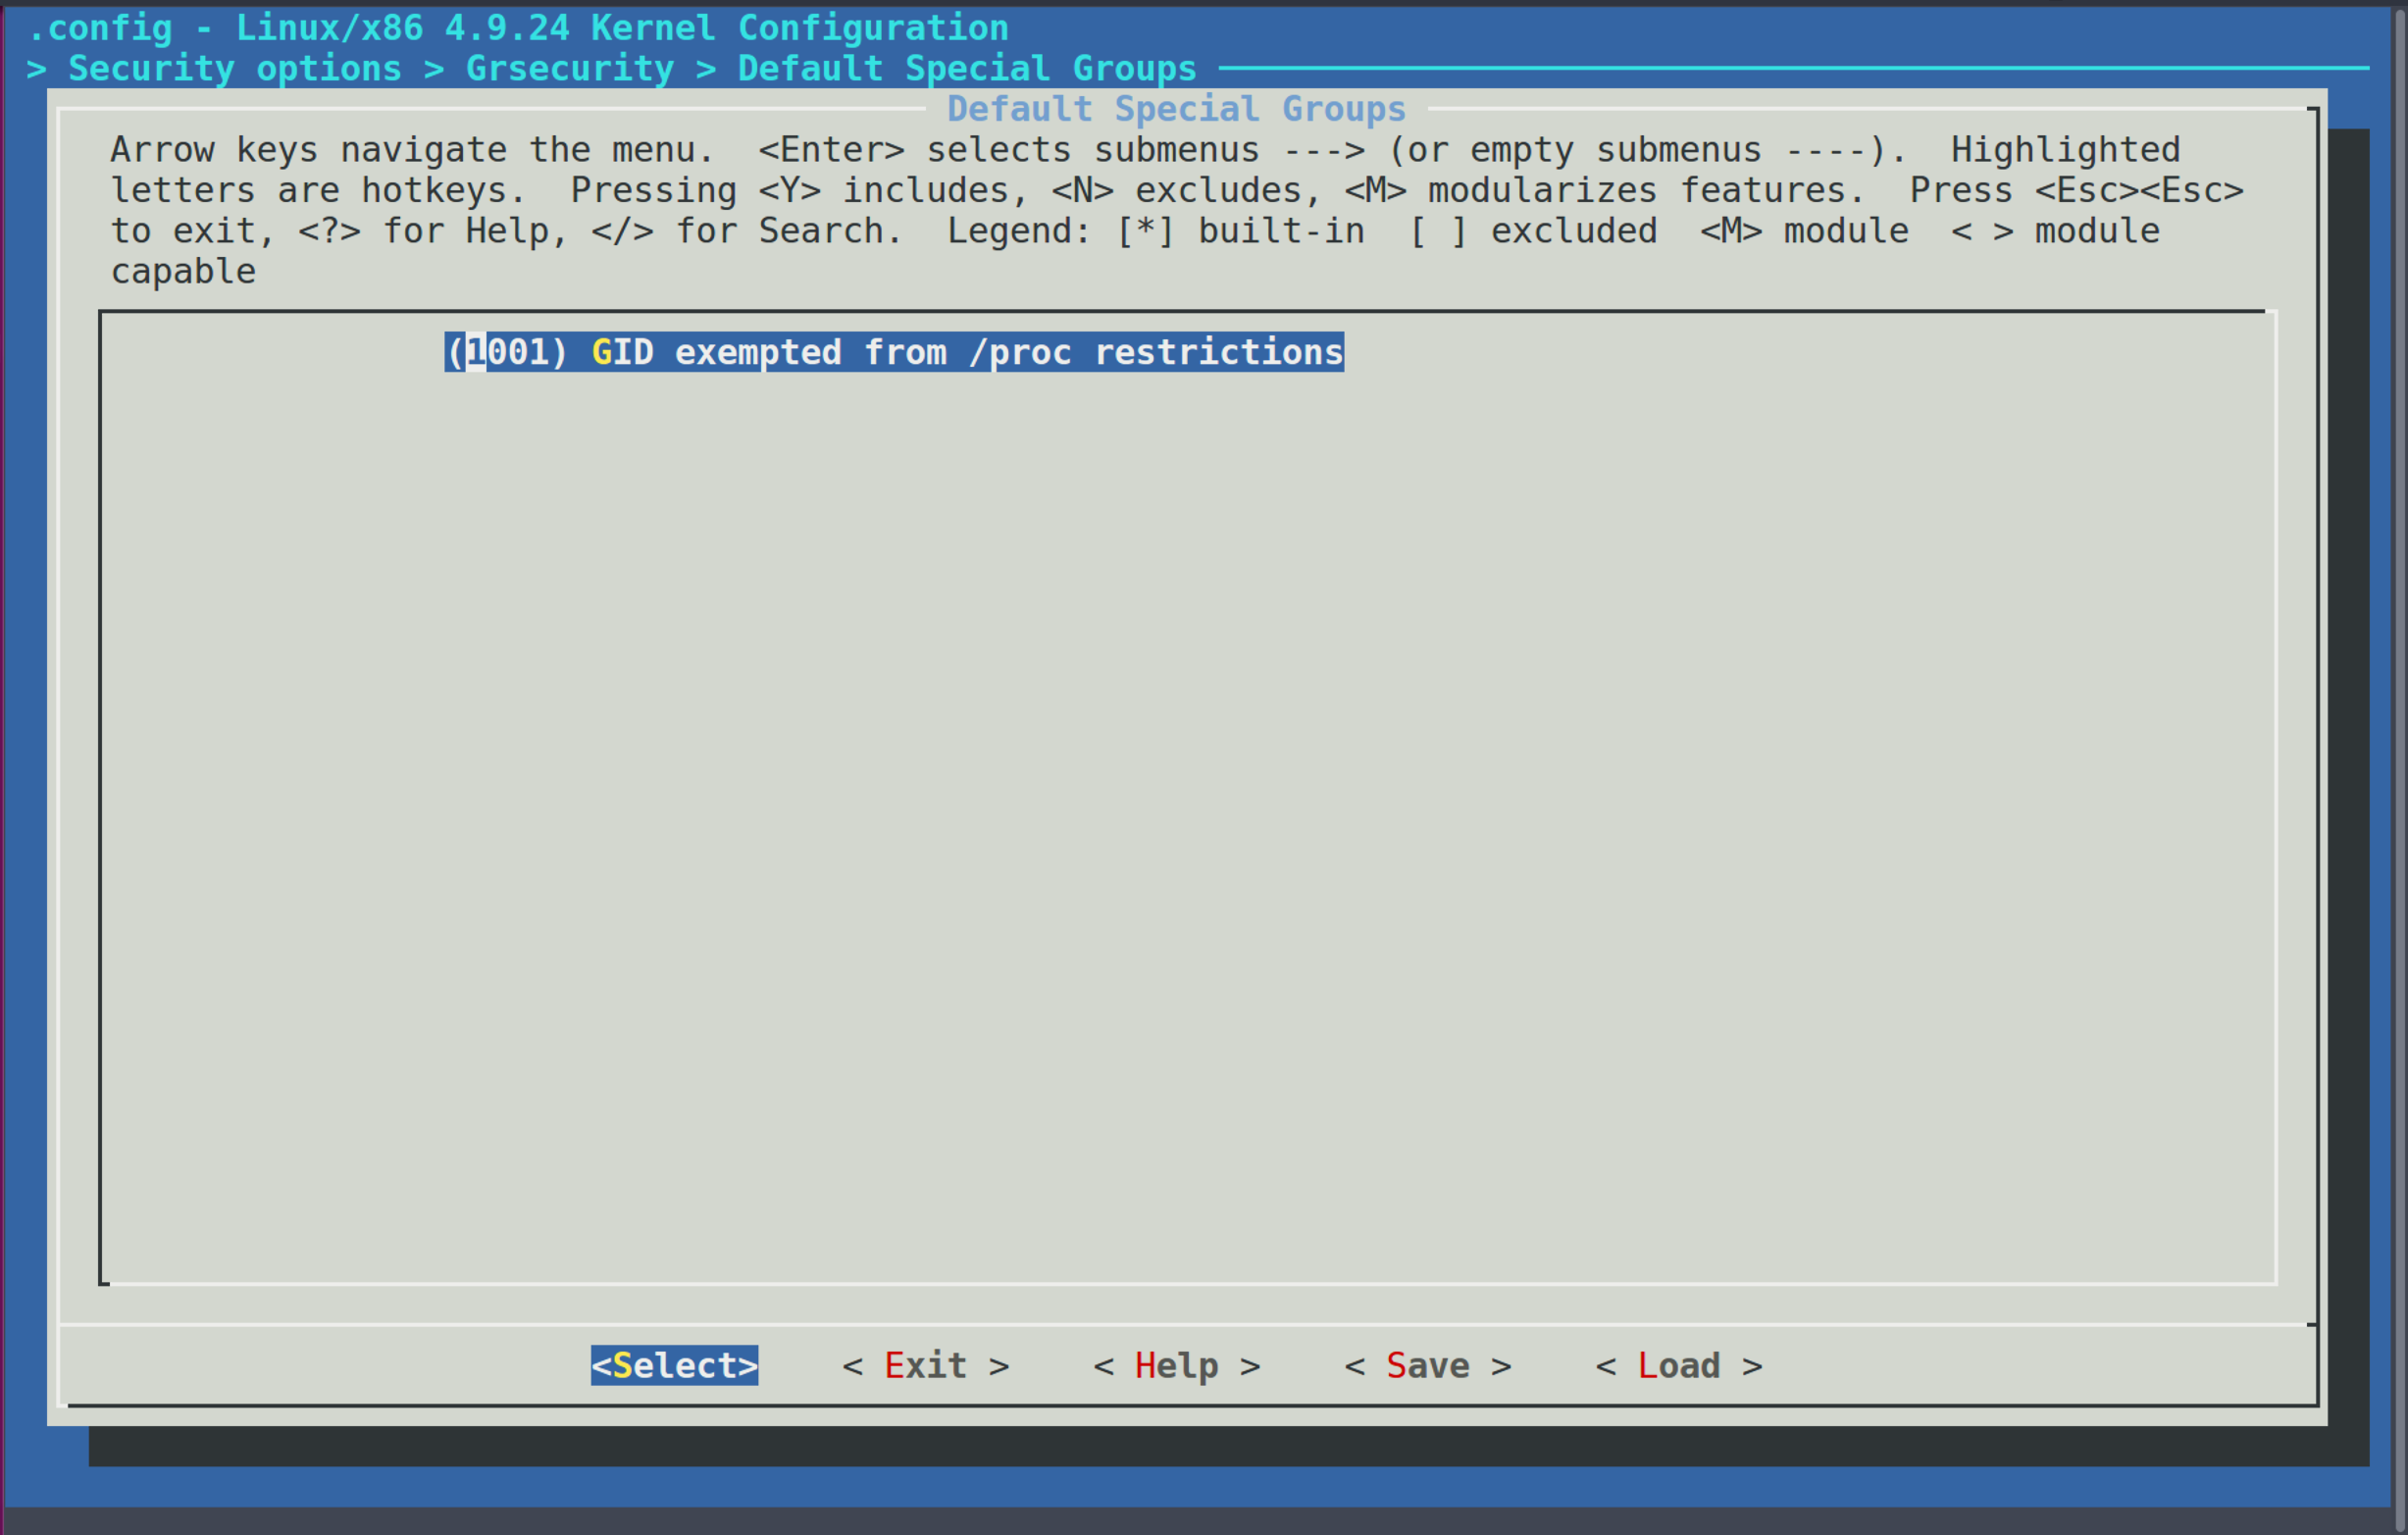
\includegraphics[width = 0.9\textwidth]{images/11.png}
\end{figure}
\begin{figure}[ht]
	\centering	
	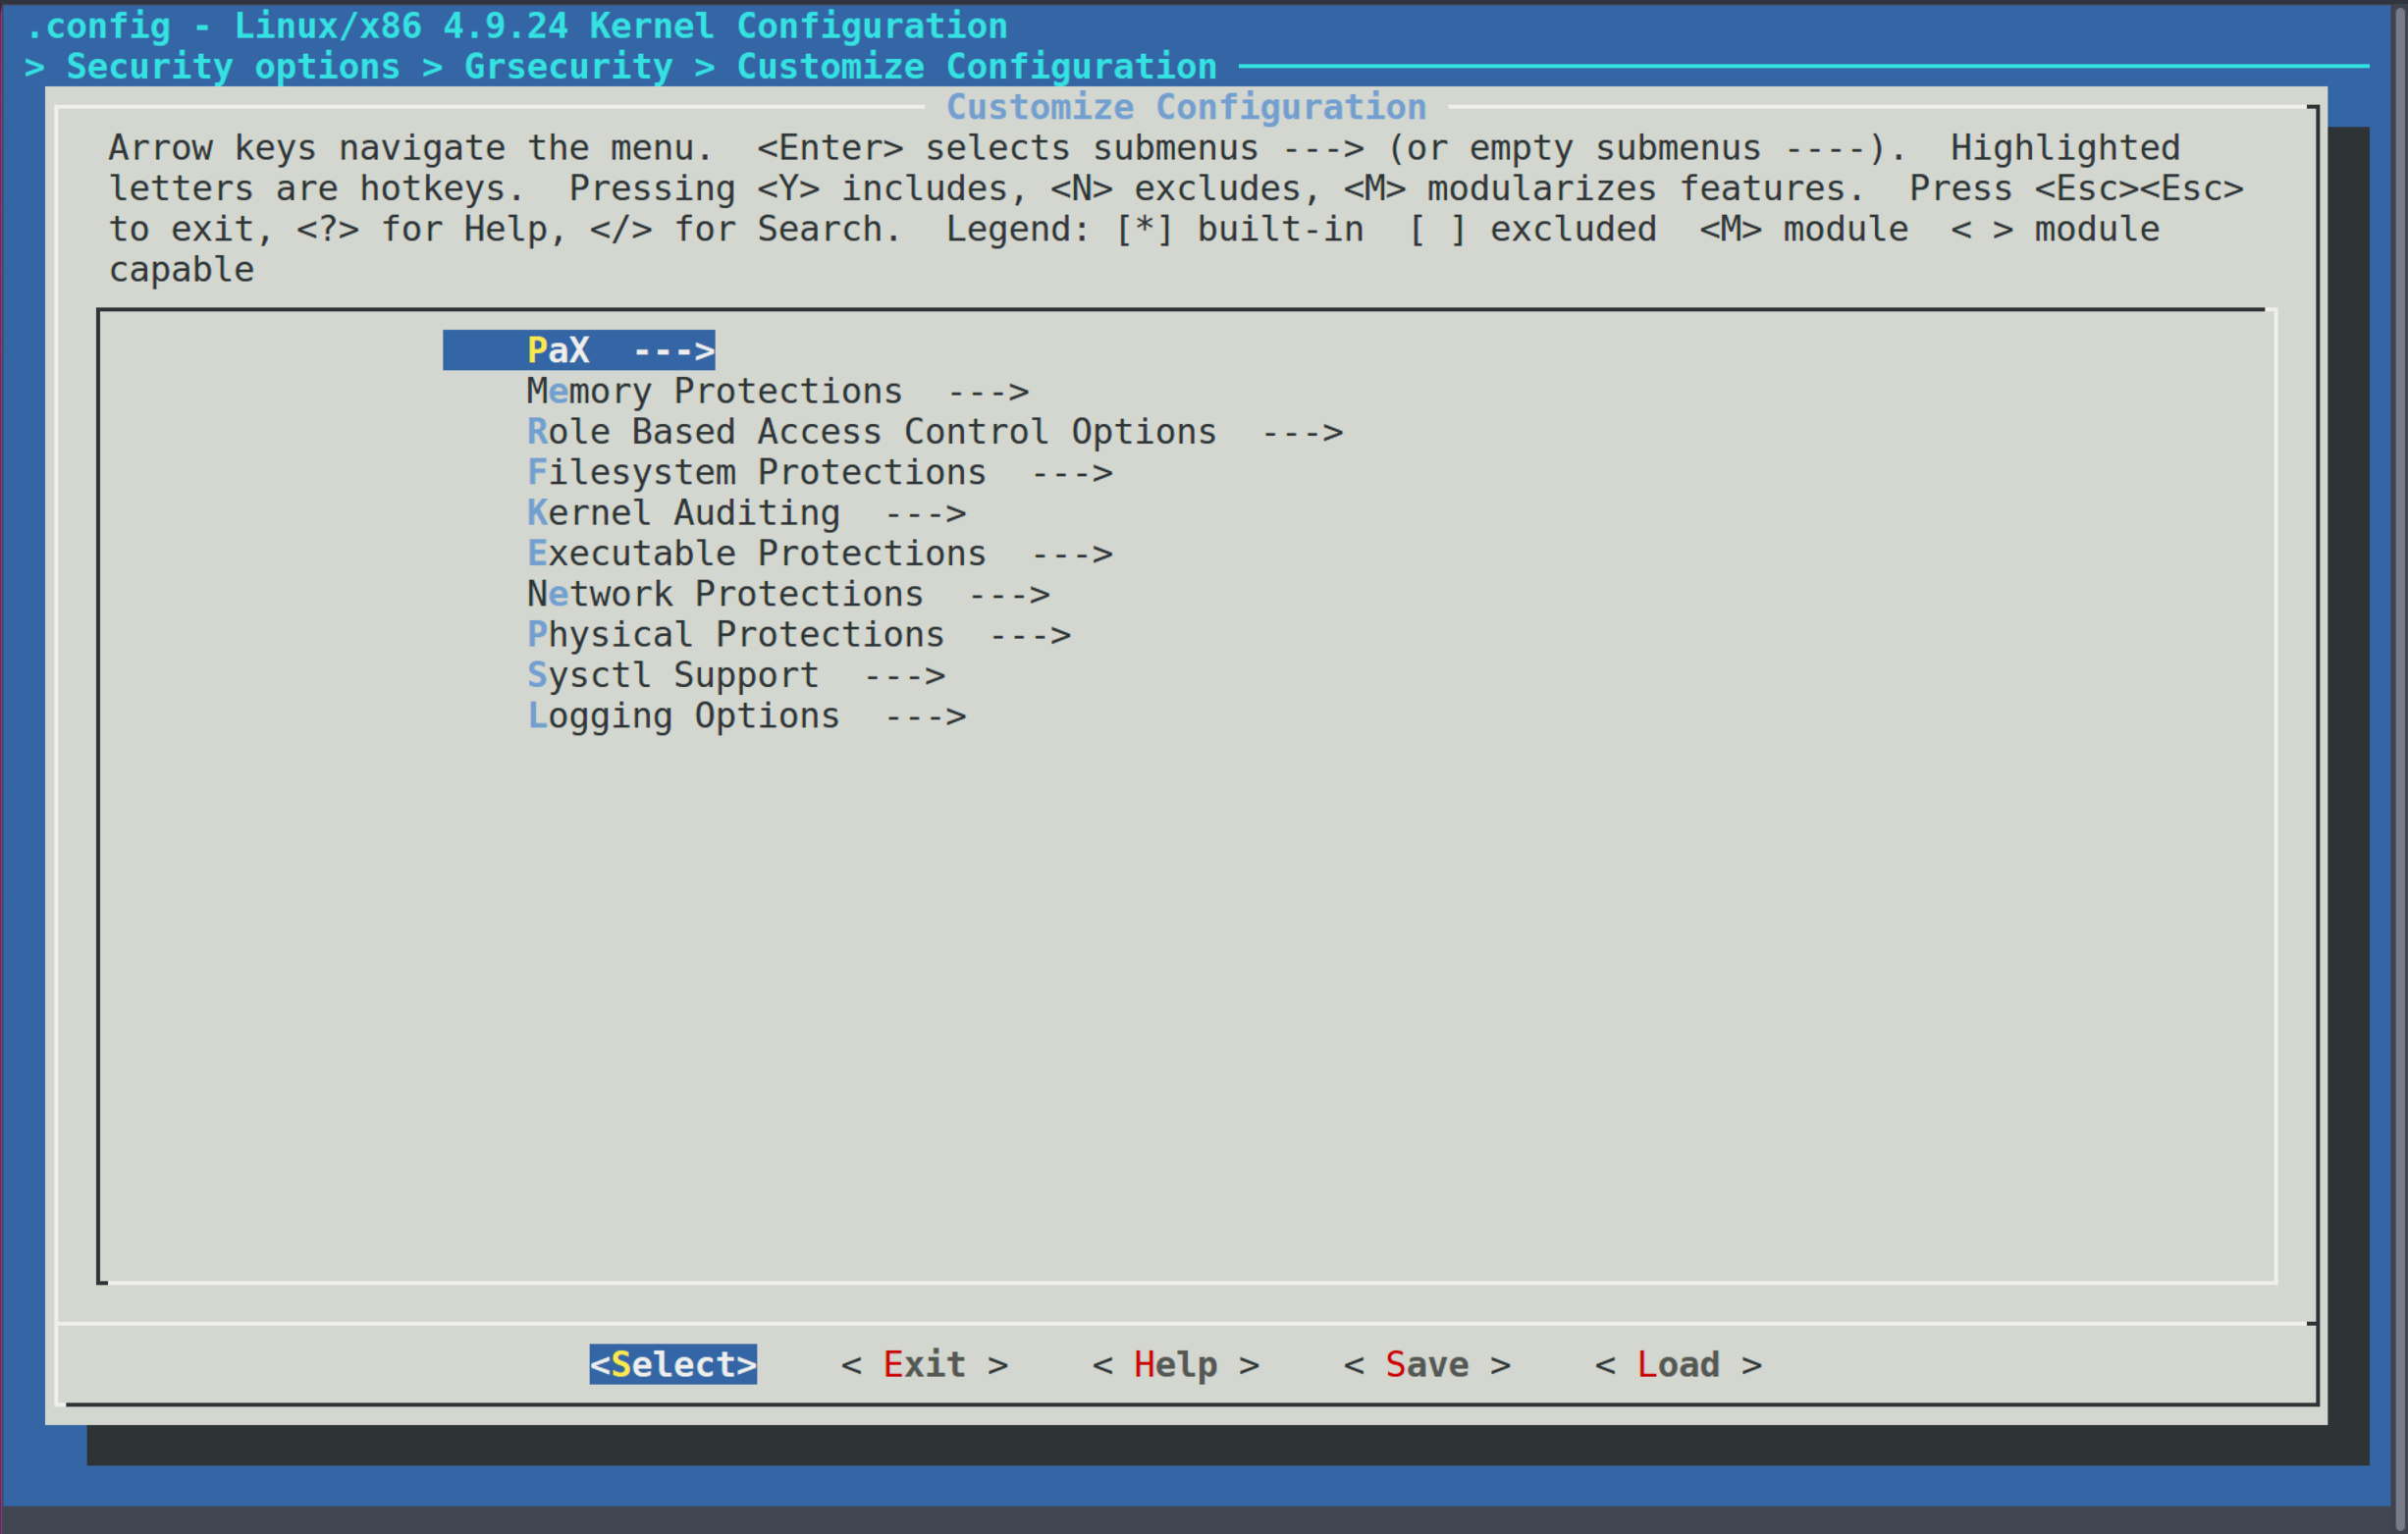
\includegraphics[width = 0.9\textwidth]{images/12.png}
\end{figure}
\newpage
سپس به دو قسمت قبل برمی‌گردیم تا SELinux را پیکربندی کنیم.
\begin{figure}[ht]
	\centering	
	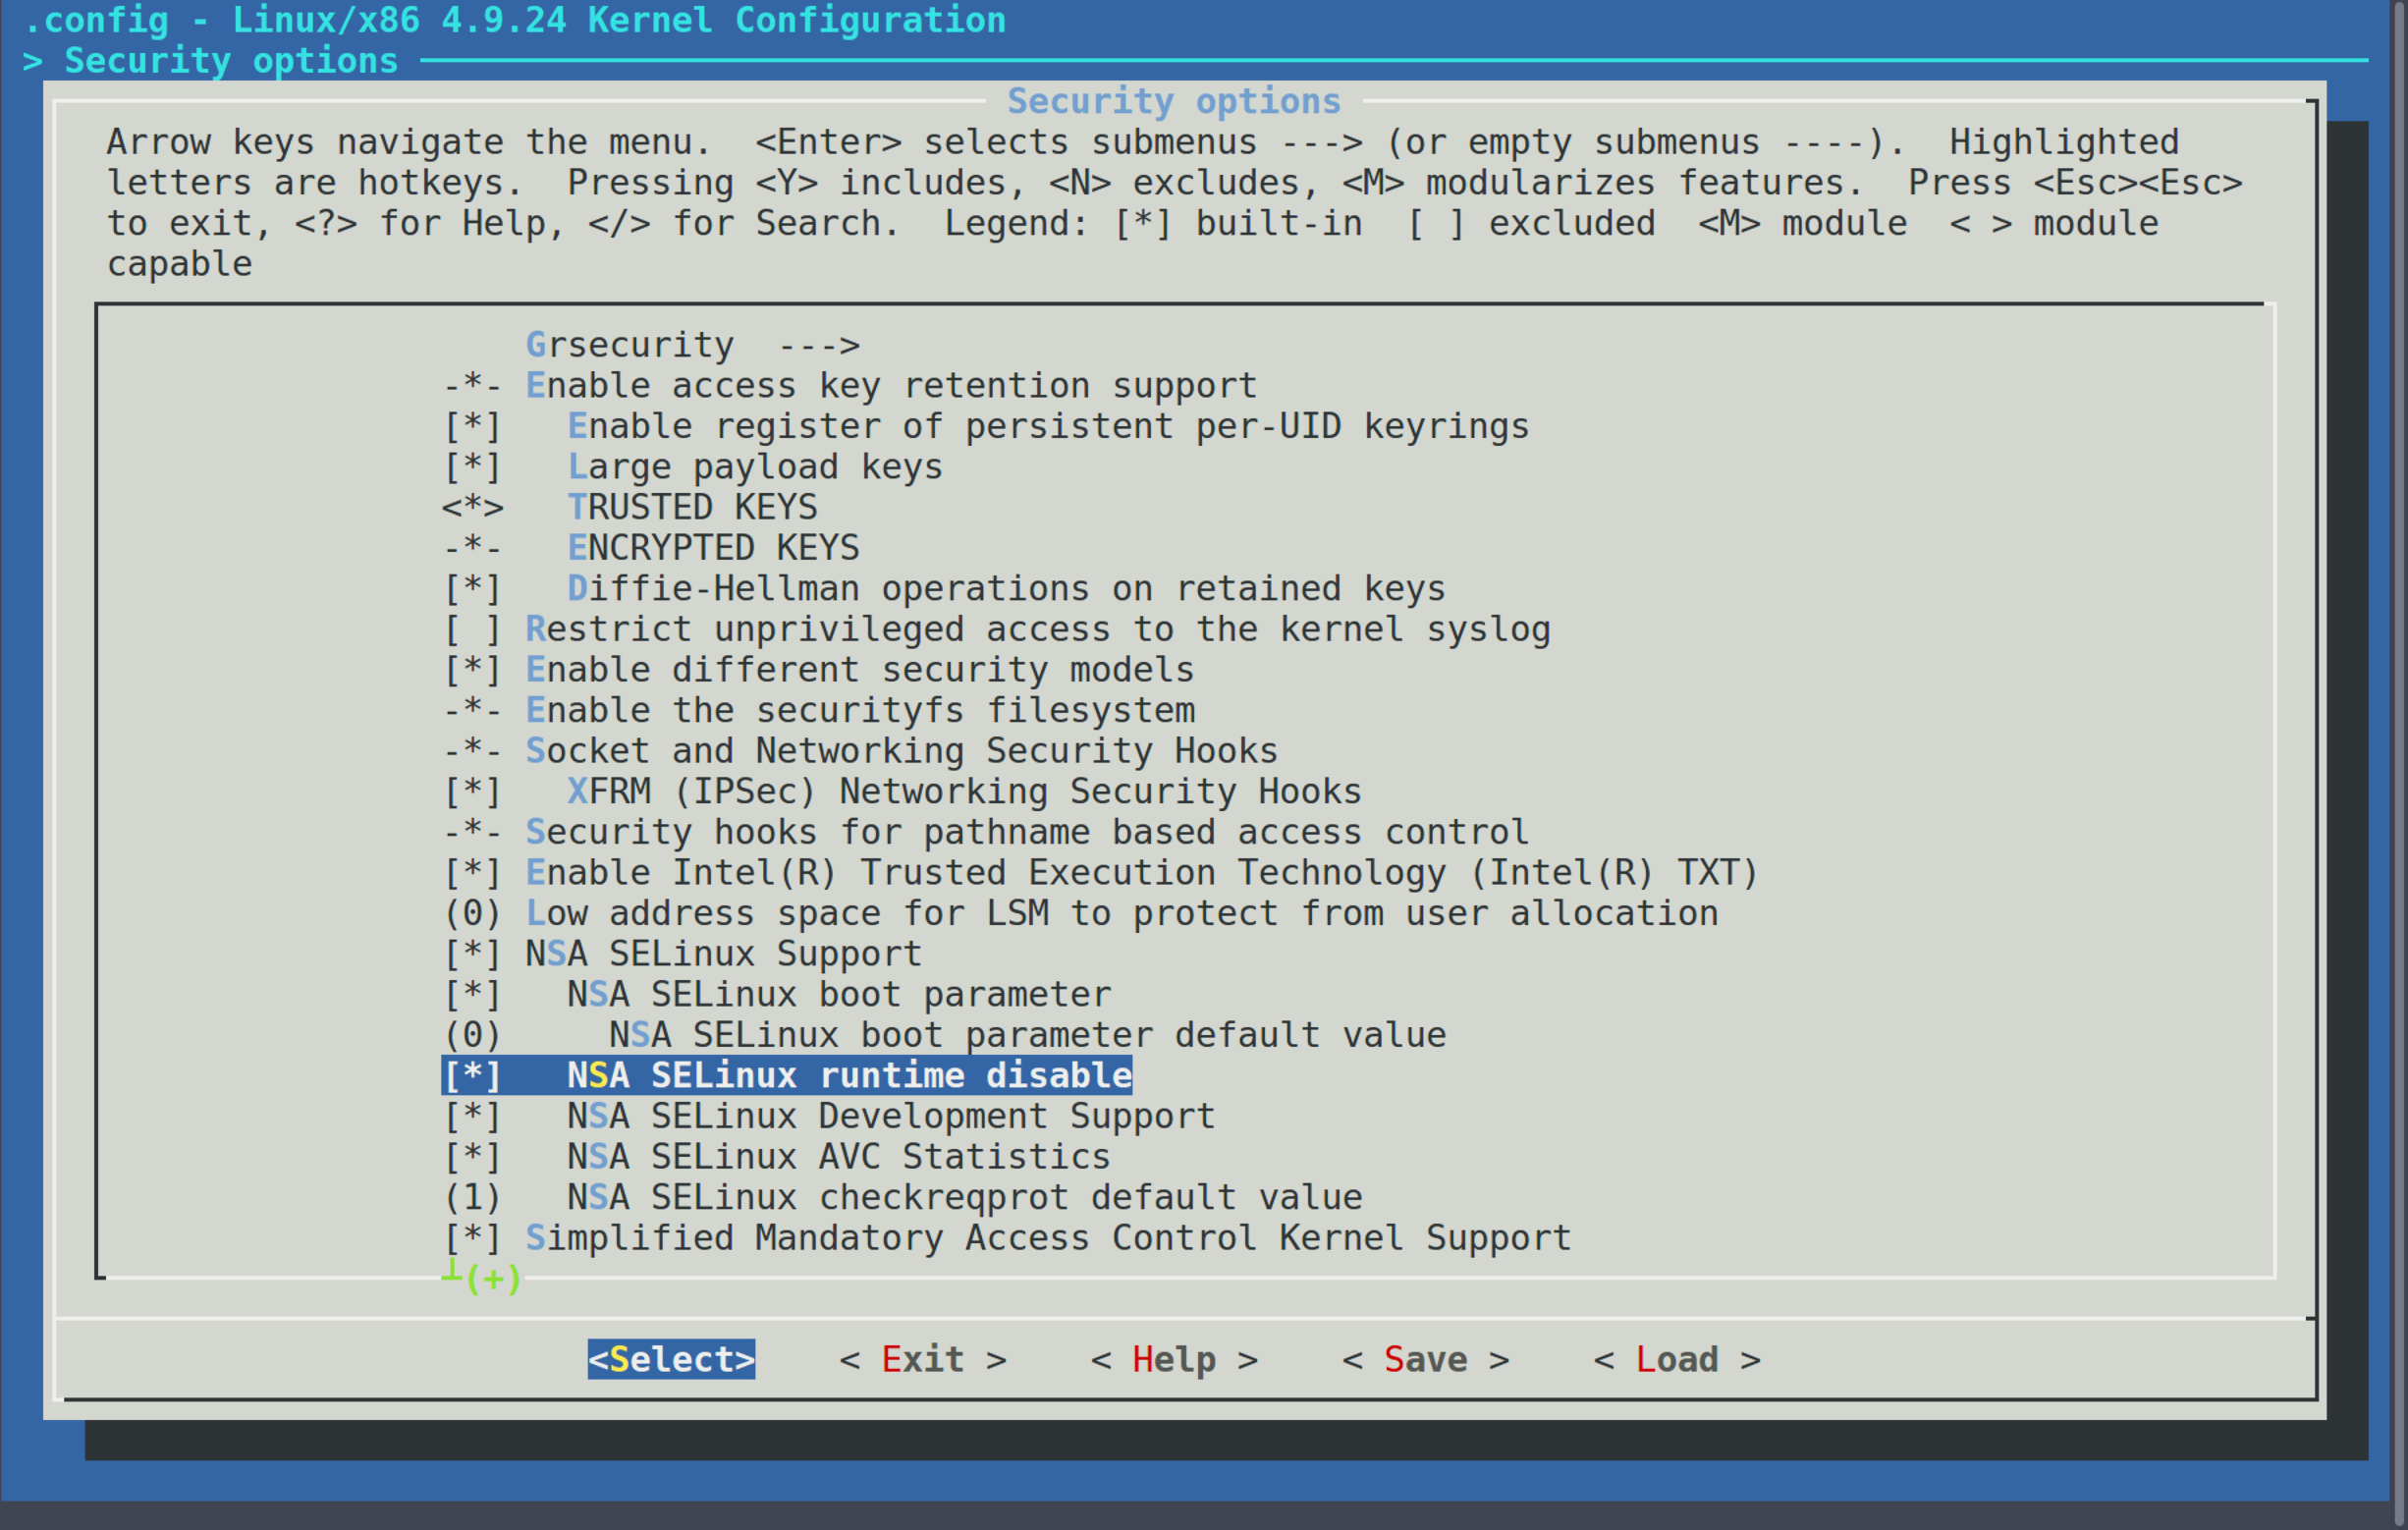
\includegraphics[width = 0.9\textwidth]{images/20.png}
\end{figure}

در این جا طبق دستورالعمل بالای صفحه وضعیت SELinux را غیرفعال می‌کنیم.

\item حال پیکربندی کرنلمان را با پیکربندی grsecurity و SELinux انجام دادیم و کرنل را با دستور زیر می‌سازیم:

\begin{latin}
\begin{verbatim}
sudo su
fakeroot make deb-pkg | tee make.txt
exit
\end{verbatim}
\end{latin}

\item حال فولدری داریم که در آن این فایل‌ها موجود هستند:
\begin{latin}
\begin{verbatim}
linux-4.9.24-grsec_4.9.24-grsec-1_amd64.changes
linux-4.9.24-grsec_4.9.24-grsec-1.debian.tar.gz
linux-4.9.24-grsec_4.9.24-grsec-1.dsc
linux-4.9.24-grsec_4.9.24-grsec.orig.tar.gz
linux-firmware-image-4.9.24-grsec_4.9.24-grsec-1_amd64.deb
linux-headers-4.9.24-grsec_4.9.24-grsec-1_amd64.deb
linux-image-4.9.24-grsec_4.9.24-grsec-1_amd64.deb
linux-image-4.9.24-grsec-dbg_4.9.24-grsec-1_amd64.deb
linux-libc-dev_4.9.24-grsec-1_amd64.deb
\end{verbatim}
\end{latin}

این فایل‌ها خروجی‌های عملیات ساختن هسته لینوکس با تغییرات اعمال شده در پیکر‌بندی هستند.

\item حال با دستور زیر تمامی این پکیج‌ها را روی سیستم نصب می‌کنیم:

\begin{latin}
\begin{verbatim}
sudo dpkg -f *.deb
\end{verbatim}
\end{latin}

\item سپس نرم‌افزار \lr{grub-customizer} را با دستور زیر نصب کرده و به وسیله‌ آن اولویت بوت سیستم را از کرنل پیش‌فرض به کرنلی که خودمان پیکر‌بندی کرده‌ایم تغییر می‌دهیم.

\begin{latin}
\begin{verbatim}
sudo apt-get install grub-customizer
sudo grub-customizer
\end{verbatim}
\end{latin}

\begin{figure}[ht]
	\centering	
	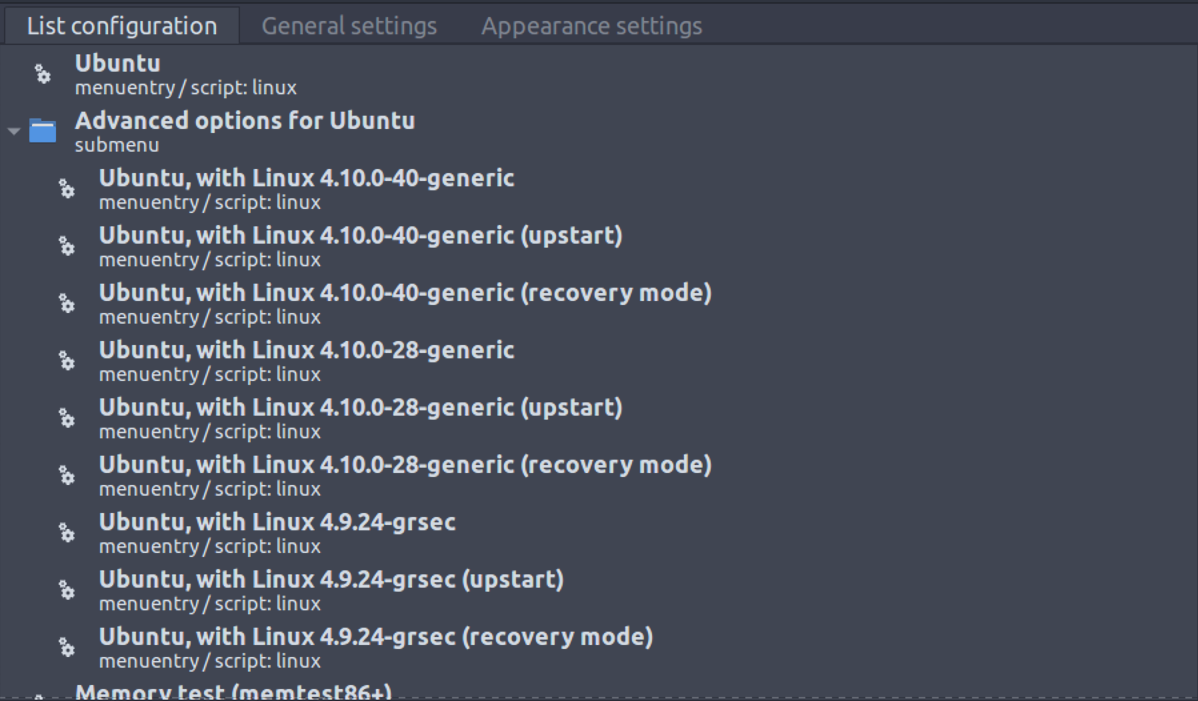
\includegraphics[width = 0.8\textwidth]{images/21.png}
\end{figure}
\begin{figure}[ht]
	\centering	
	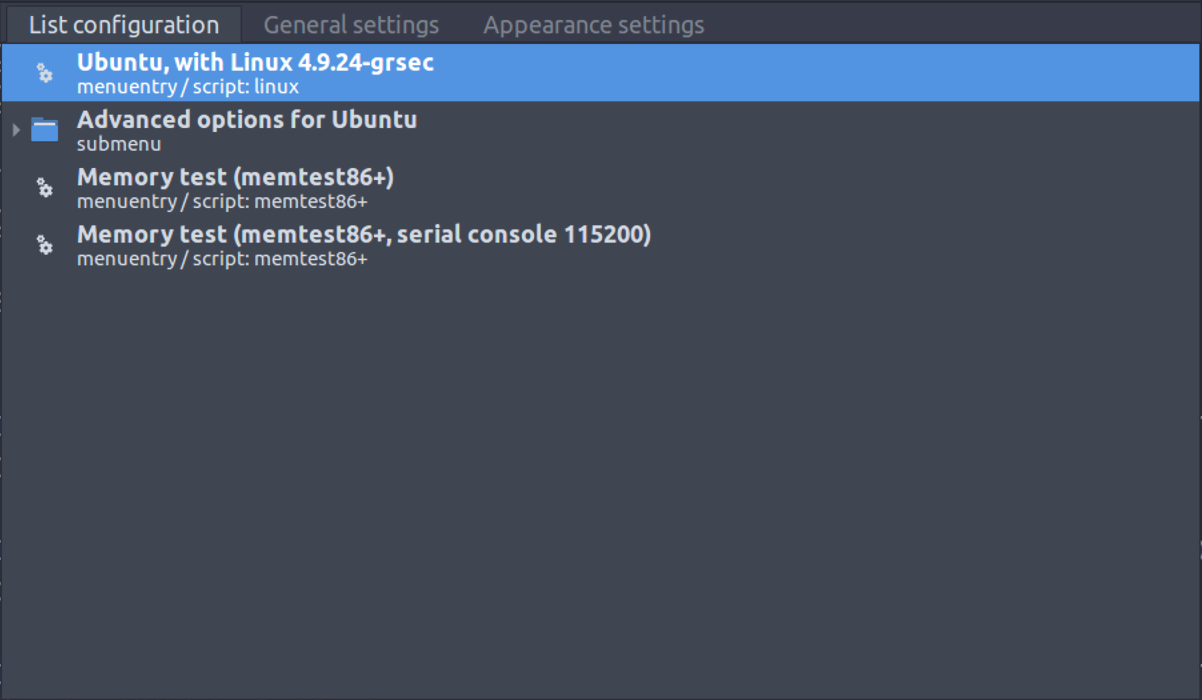
\includegraphics[width = 0.8\textwidth]{images/22.png}
\end{figure}

\item سپس سیستم را مجددا بوت می‌کنیم و پس از بوت کردن مجددا ابتدا پکیج sestatus و paxtest را نصب می‌‌کنیم تا وضعیت SELinux و grsecurity را بررسی کنیم.

\begin{latin}
\begin{verbatim}
sudo apt-get install sestatus
sudo apt-get install paxtest
\end{verbatim}
\end{latin}

\item با زدن دستور sestatus سیستم وضعیت SELinux را به ما گزارش می‌کند و چنین خروجی می‌دهد:

\begin{latin}
\begin{verbatim}
sestatus
SELinux status:		disabled
\end{verbatim}
\end{latin}

\item سپس دستور زیر را اجرا می‌کنیم تا تعدادی از عملیات‌های خطرناک و غیرامن را شبیه‌سازی کرده و واکنش سیستم نسبت به آن‌ها را ببینیم:
\begin{latin}
\begin{verbatim}
paxtest kiddie
\end{verbatim}
\end{latin}
می‌بینیم که در ادامه سیستم تعداد زیادی پیغام خطا به شکل زیر چاپ شده و خروجی زیر در ترمینال چاپ می‌شود:
\begin{figure}[ht]
	\centering	
	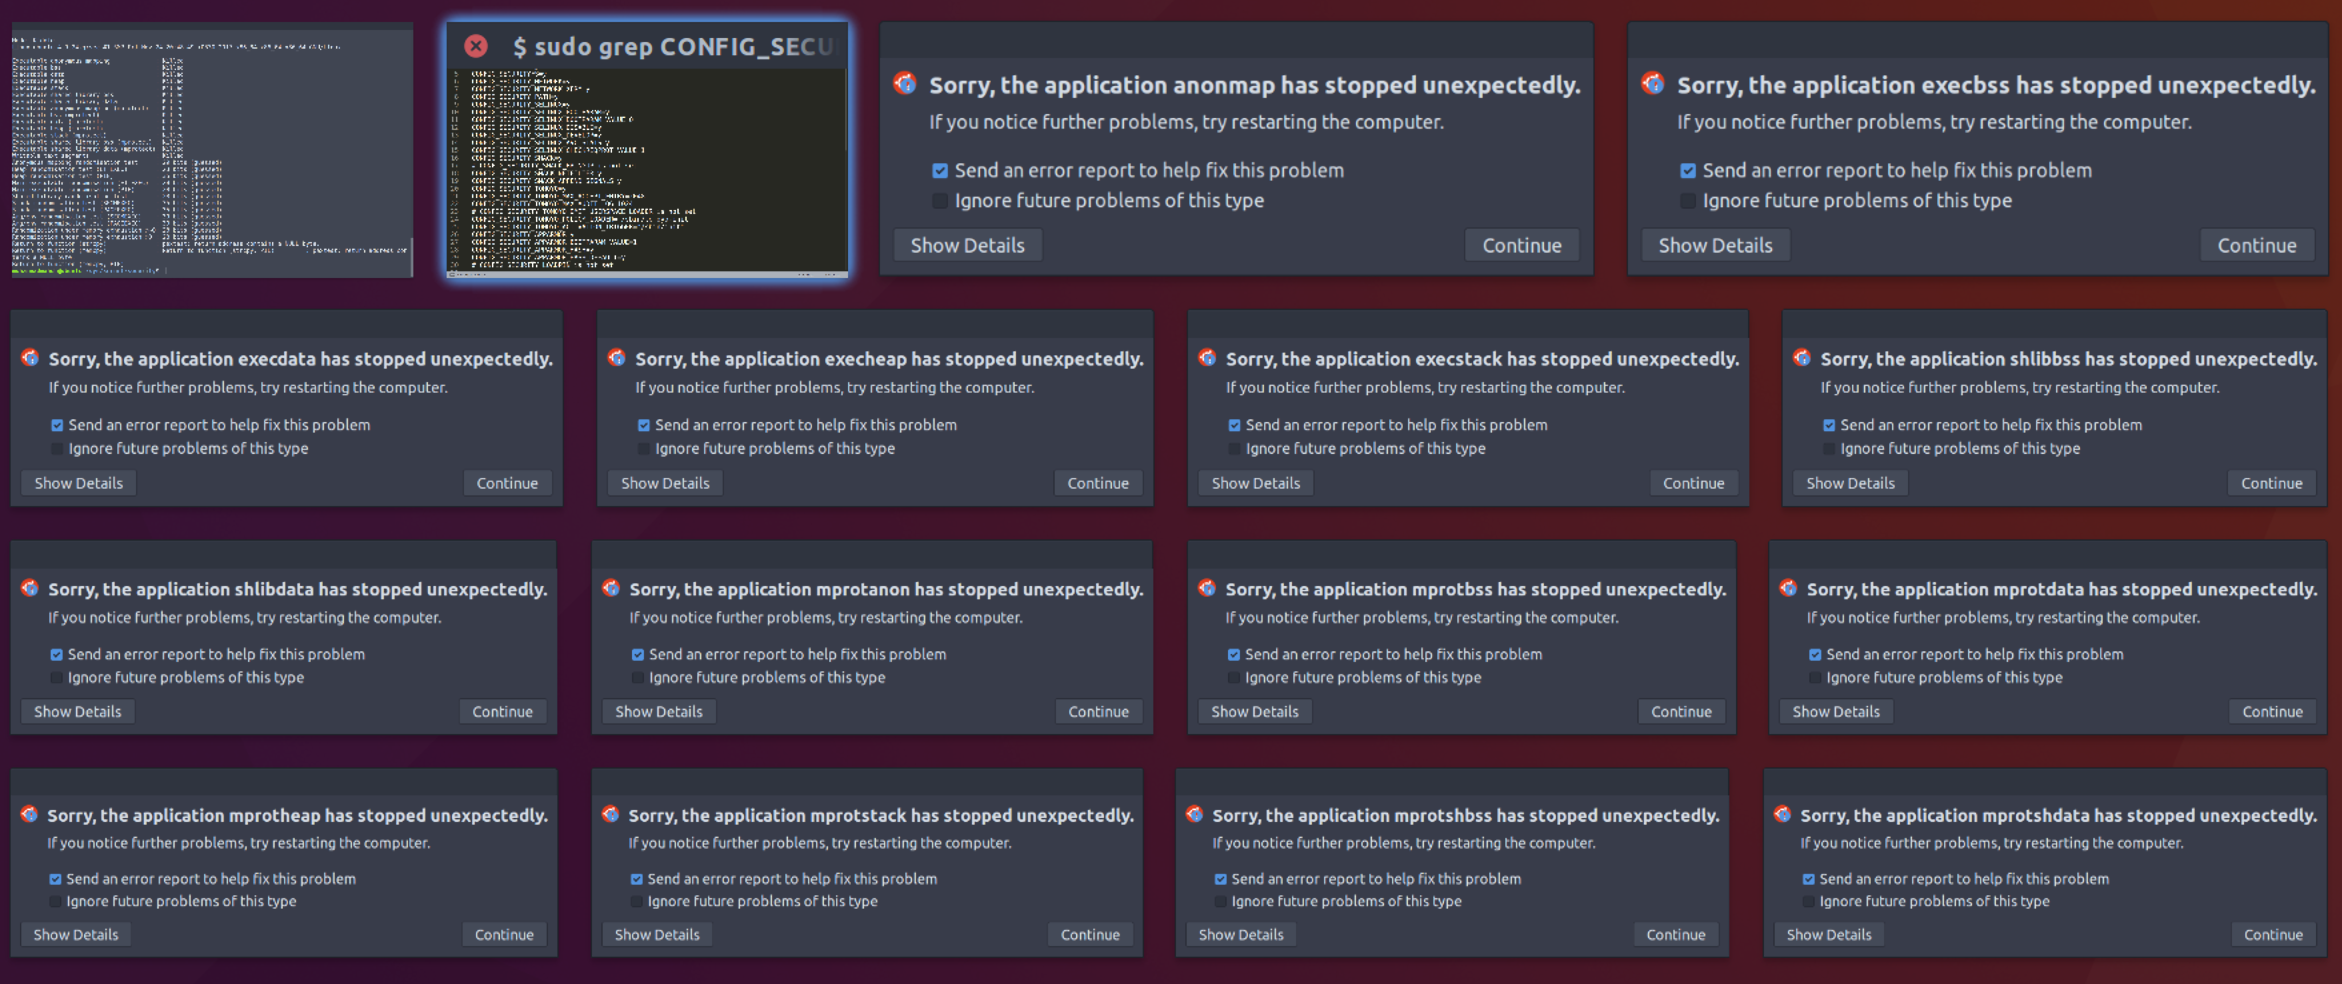
\includegraphics[width = 1\textwidth]{images/23.png}
\end{figure}
\begin{latin}
\begin{verbatim}
PaXtest - Copyright(c) 2003,2004 by Peter Busser <peter@adamantix.org>
Released under the GNU Public Licence version 2 or later

Writing output to /home/mohammadmahdi/paxtest.log
It may take a while for the tests to complete
Test results:
PaXtest - Copyright(c) 2003,2004 by Peter Busser <peter@adamantix.org>
Released under the GNU Public Licence version 2 or later

Mode: Kiddie
Linux ubuntu 4.9.24-grsec #1 \
 SMP Fri Nov 24 20:48:49 +0330 2017 x86_64 x86_64 x86_64 GNU/Linux

Executable anonymous mapping             : Killed
Executable bss                           : Killed
Executable data                          : Killed
Executable heap                          : Killed
Executable stack                         : Killed
Executable shared library bss            : Killed
Executable shared library data           : Killed
Executable anonymous mapping (mprotect)  : Killed
Executable bss (mprotect)                : Killed
Executable data (mprotect)               : Killed
Executable heap (mprotect)               : Killed
Executable stack (mprotect)              : Killed
Executable shared library bss (mprotect) : Killed
Executable shared library data (mprotect): Killed
Writable text segments                   : Killed
Anonymous mapping randomisation test     : 28 bits (guessed)
Heap randomisation test (ET_EXEC)        : 23 bits (guessed)
Heap randomisation test (PIE)            : 35 bits (guessed)
Main executable randomisation (ET_EXEC)  : 28 bits (guessed)
Main executable randomisation (PIE)      : 28 bits (guessed)
Shared library randomisation test        : 28 bits (guessed)
Stack randomisation test (SEGMEXEC)      : 35 bits (guessed)
Stack randomisation test (PAGEEXEC)      : 35 bits (guessed)
Arg/env randomisation test (SEGMEXEC)    : 39 bits (guessed)
Arg/env randomisation test (PAGEEXEC)    : 39 bits (guessed)
Randomization under memory exhaustion @~0: 28 bits (guessed)
Randomization under memory exhaustion @0 : 28 bits (guessed)
Return to function (strcpy) \
: paxtest: return address contains a NULL byte.
Return to function (memcpy) \
: Return to function (strcpy, PIE) \
: paxtest: return address contains a NULL byte.
Return to function (memcpy, PIE)

\end{verbatim}
\end{latin}
که این نشان از این دارد که پیکربندی grsecurity به درستی انجام شده است.

\end{enumerate}

اسکریپت اتوماسیون شده این عملیات به وسیله تراویس نیز در فایل .travis.yml در مخزن گیت‌هاب موجود است.


\section*{گام سوم: ساخت rom اندروید برای گوشی موبایل\lr{Nexus 5x}}
 ابتدا پکیج‌های مورد نیاز فرایند ساخت را با دستورات زیر نصب می‌کنیم:
 
\begin{latin}
\begin{verbatim}
$ sudo apt install bison build-essential curl flex git gnupg gperf \
  libesd0-dev liblz4-tool libncurses5-dev libsdl1.2-dev ibwxgtk3.0-dev \
  libxml2 libxml2-utils lzop maven pngcrush schedtool squashfs-tools \
  xsltproc zip lib32readline-gplv2-dev zlib1g-dev g++-multilib gcc-multilib \
  lib32ncurses5-dev  lib32z1-dev

$ sudo apt install rsync
\end{verbatim}	
\end{latin}
سپس فایلی را که از ftp سرور دانشگاه دانلود کردیم را با این دستورات به پوشه‌ی خانگی منتقل کرده و از حالت فشرده خارج می‌کنیم:
\begin{latin}
\begin{verbatim}
$ mv ~/Downloads/android.tar ~/
$ cd ~/
$ tar -xvf android.tar | tee source_unpack.txt
\end{verbatim}	
\end{latin}
حال ابزار repo را از سرور گوگل دانلود کرده و در پوشه‌ی bin ذیل پوشه‌ی خانگی قرار می‌دهیم:
\begin{latin}
\begin{verbatim}
$ mkdir -p ~/bin
$ curl https://storage.googleapis.com/git-repo-downloads/repo > ~/bin/repo
$ chmod a+x ~/bin/repo
\end{verbatim}	
\end{latin}

سپس فایل profile را ذیل پوشه‌ی خانگی ویرایش کرده و این خطوط را به آن اضافه می‌کنیم:

\begin{latin}
\begin{verbatim}
$ gedit ~/.profile
+ if [ -d "$HOME/bin" ] ; then
+    PATH="$HOME/bin:$PATH"
+ fi
\end{verbatim}	
\end{latin}

حالا محیط را برای دانلود کرنل و تنظیمات ساخت آماده می‌کنیم. وارد پوشه‌ی ریشه‌ی کد منبع می‌شویم. دستورات زیر را اجرا می‌کنیم:

\begin{latin}
\begin{verbatim}
$ cd ~/android/lineage/
$ source ~/.profile
$ source build/envsetup.sh
\end{verbatim}	
\end{latin}
خروجی دستور آخر اینگونه است:
\begin{latin}
\begin{verbatim}
> including device/generic/mini-emulator-arm64/vendorsetup.sh
  including device/generic/mini-emulator-armv7-a-neon/vendorsetup.sh
  including device/generic/mini-emulator-x86_64/vendorsetup.sh
  including device/generic/mini-emulator-x86/vendorsetup.sh
  including vendor/cm/vendorsetup.sh
  including sdk/bash_completion/adb.bash
  including vendor/cm/bash_completion/git.bash
  including vendor/cm/bash_completion/repo.bash
\end{verbatim}	
\end{latin}

حالا دستور زیر را اجرا می‌کنیم تا کرنل و تنظیمات مورد نیاز برای ساخت دانلود شوند. لازم به ذکر است با این دستور فایل لاگی از تمام خروجی‌های گرفته شده هم ساخته خواهد شد:
\begin{latin}
\begin{verbatim}
$ breakfast bullhead | tee breakfast_log.txt
\end{verbatim}
\end{latin}
لازم به ذکر است اجرای این دستور ۳۲ دقیقه طول کشید.
محیط را برای عملیات ساخت آماده می‌کنیم. 
استفاده از کامپایلر NINJA را غیر فعال می‌کنیم تا با خطا‌های احتمالی ناشی از پیکربندی نادرست آن رو به رو نشویم.

\begin{latin}
\begin{verbatim}
$ export USE_NINJA=false
\end{verbatim}
\end{latin}

برای کاهش زمان ساخت ۵۰ گیگابایت فضای cache به سیستم ساخت تخصیص می‌دهیم:
\begin{latin}
\begin{verbatim}
$ export USE_CCACHE=1
$ prebuilts/misc/linux-x86/ccache/ccache -M 50G
\end{verbatim}
\end{latin}
برای بر نخوردن به مشکل کمبود حافظه هنگام ساخت، حافظه‌ی تخضیص داده شده به سیستم ساخت را به ۴ گیگابایت افزایش می‌دهیم:
\begin{latin}
\begin{verbatim}
$ export ANDROID_JACK_VM_ARGS="-Dfile.encoding=UTF-8 -XX:+TieredCompilation -Xmx4G"
\end{verbatim}
\end{latin}
حالا عملیات ساخت را شروع می‌کنیم. لازم به ذکر است با این دستور فایل لاگی از تمام خروجی‌های گرفته شده هم ساخته خواهد شد:
\begin{latin}
\begin{verbatim}
$ croot
$ brunch bullhead | tee brunch_log.txt
\end{verbatim}
\end{latin}
اجرای این دستور روی یک پردازنده‌ی ۲ هسته‌ای \lr{Intel core i7 3537U}  با هر دو هسته‌ی پردازشی، ۵۰ گیگابایت کش و ۴ گیگابایت رم اختصاصی، نزدیک به ۷ ساعت به طول انجامید.

در انتها به مسیر فایل‌های خروجی رفته و آنها را مشاهده می‌کنیم:
\begin{latin}
\begin{verbatim}
$ cd ~/android/lineage/out/target/product/bullhead
$ ls
\end{verbatim}
\end{latin}
این فایل‌ها چنین هستند:
\begin{latin}
\begin{verbatim}
android-info.txt       
installed-files.txt                                          
ramdisk-recovery.img
boot.img               
kernel                                                       
recovery
build_fingerprint.txt  
lineage-14.1-20171203_183811-UNOFFICIAL-bullhead.zip         
recovery.id
cache                  
lineage-14.1-20171203_183811-UNOFFICIAL-bullhead.zip.md5sum  
recovery.img
cache.img              
lineage_bullhead-ota-73e82086d6.zip                          
root
clean_steps.mk         
obj                                                          
symbols
data                   
obj_arm                                                      
system
fake_packages          
ota_script_path                                              
system.img
gen                    
previous_build_config.mk                                     
userdata.img
install                
ramdisk.img
installed-files.json   
ramdisk-recovery.cpio
\end{verbatim}
\end{latin}

لازم به ذکر است که خروجی‌های ساخت و زیر تمامی log ها در مخزن گیت پروژه قرار گرفته است. تنها نمی‌توانستیم فایل‌های zip نهایی rom را به علت حجم بالایشان روی مخزن قرار دهیم که در تحویل حضوری پروژه حضورا تحویل خواهند شد.

\begin{thebibliography}{9}

\latin
\bibitem{1}
\url{http://www.thegeekstuff.com/2013/07/write-linux-kernel-module/?utm_source=tuicool}
\bibitem{2}
\url{https://stackoverflow.com/questions/10476990/difference-between-o-and-ko-file}
\bibitem{3}
\url{https://askubuntu.com/questions/20070/whats-the-difference-between-insmod-and-modprobe}
\bibitem{4}
\url{https://unix.stackexchange.com/questions/47330/what-exactly-are-linux-kernel-headers}
\bibitem{5}
\url{https://wiki.lineageos.org/devices/bullhead/build}

\end{thebibliography}

\end{document}